\chapter{Methods}\label{sec:methods}
In this chapter, the methods for investigating a bridge design, verifying its structural safety and estimating its cost are introduced. In \cref{sec:met_ref} the Blennerhassett Island Bridge and other reference bridges are presented.
\cref{sec:met_str} introduces the structural model and briefly assesses its underlying assumptions. 
Further, an overview of the investigated load cases is given in \cref{sec:met_loads}. 
The self-equilibrium stress state is a fundamental factor for designing an optimised network tied-arch bridge and is presented in \cref{sec:met_seq}.
It partially overlaps with the choice of an efficient arch shape presented in \cref{sec:met_arch}.
The limit states for the design criteria and the corresponding verifications are specified in \cref{sec:met_ver}, combining the self-equilibrium stress state with the factored load cases. Based on these verifications, an investigated design's cost is estimated according to \cref{sec:met_cost}. The methods are exemplified by the final design of the Blennerhassett Island Bridge.

\section{Reference bridges} \label{sec:met_ref}
The main focus of this Thesis lies in the investigation of the Blennerhassett Island Bridge. It is introduced in detail in \cref{sec:Blennerhassett}. Further, other network tied-arch bridges are summarised in \cref{sec:other_bridges} to enhance the understanding of the Blennerhassett Island Bridge's particularities. This will allow evaluating the results in a broader perspective.
\subsection{Blennerhassett Island Bridge}\label{sec:Blennerhassett}
The Blennerhassett Island Bridge overpasses the Ohio River near Parkersburg (West Virginia) and was completed in 2008. Along with the Providence River Bridge, it was the first network tied-arch bridge built in the United States. The entire bridge is \SI{1222}{m} long of which the tied-arch spans \SI{267.8}{m} across the navigable channel of the Ohio River as shown in \cref{fig:Blennerhassett_2_5}. This made it the second-longest bridge of this type at the time. 
The network arrangement, shown in \cref{fig:Blennerhassett_1}, was chosen over the traditional vertical arrangement for it increases stiffness, strength and redundancy of the structure \cite{Wollmann}.

\begin{figure}[H]
\centering
\begin{subfigure}{.5\textwidth}
    \centering
    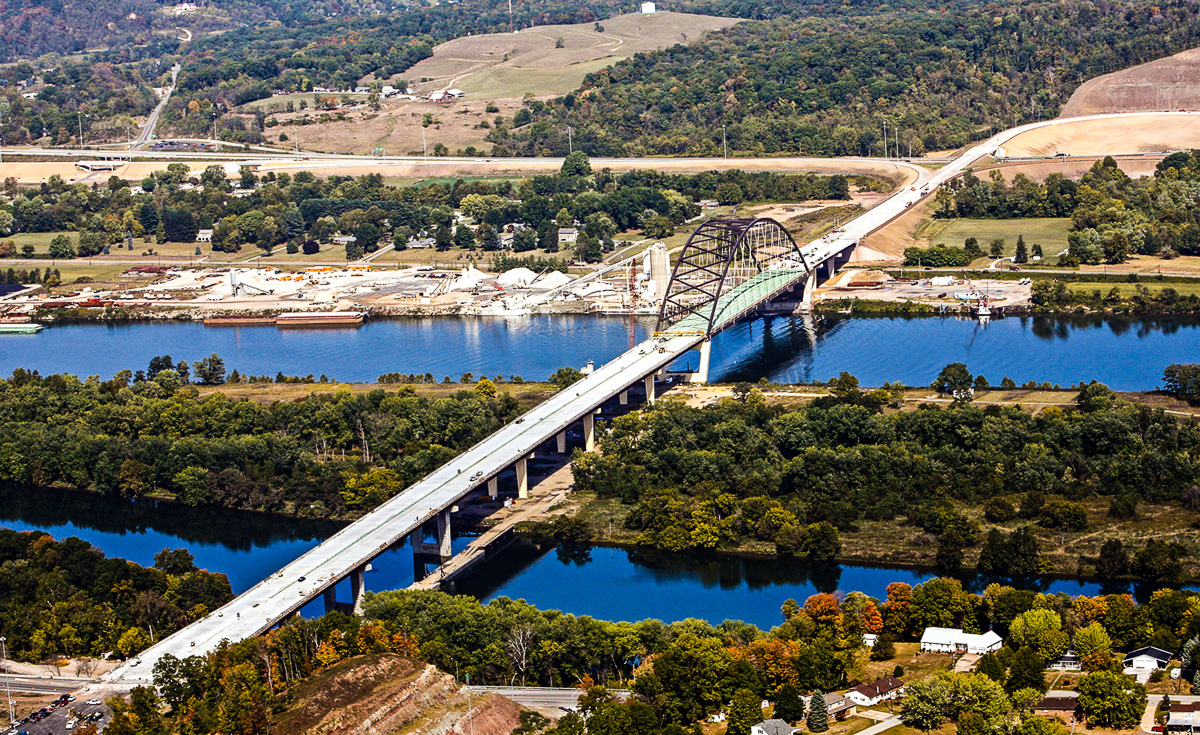
\includegraphics[trim={0 0.4cm 0 0},clip, width=0.9\textwidth]{overleaf/Pictures/Blennerhassett_3.jpg}
    \caption{Construction site (adapted from \cite{Blennerhassett})}
    \label{fig:Blennerhassett_2_5}
\end{subfigure}%
\begin{subfigure}{0.5\textwidth}
    \centering
    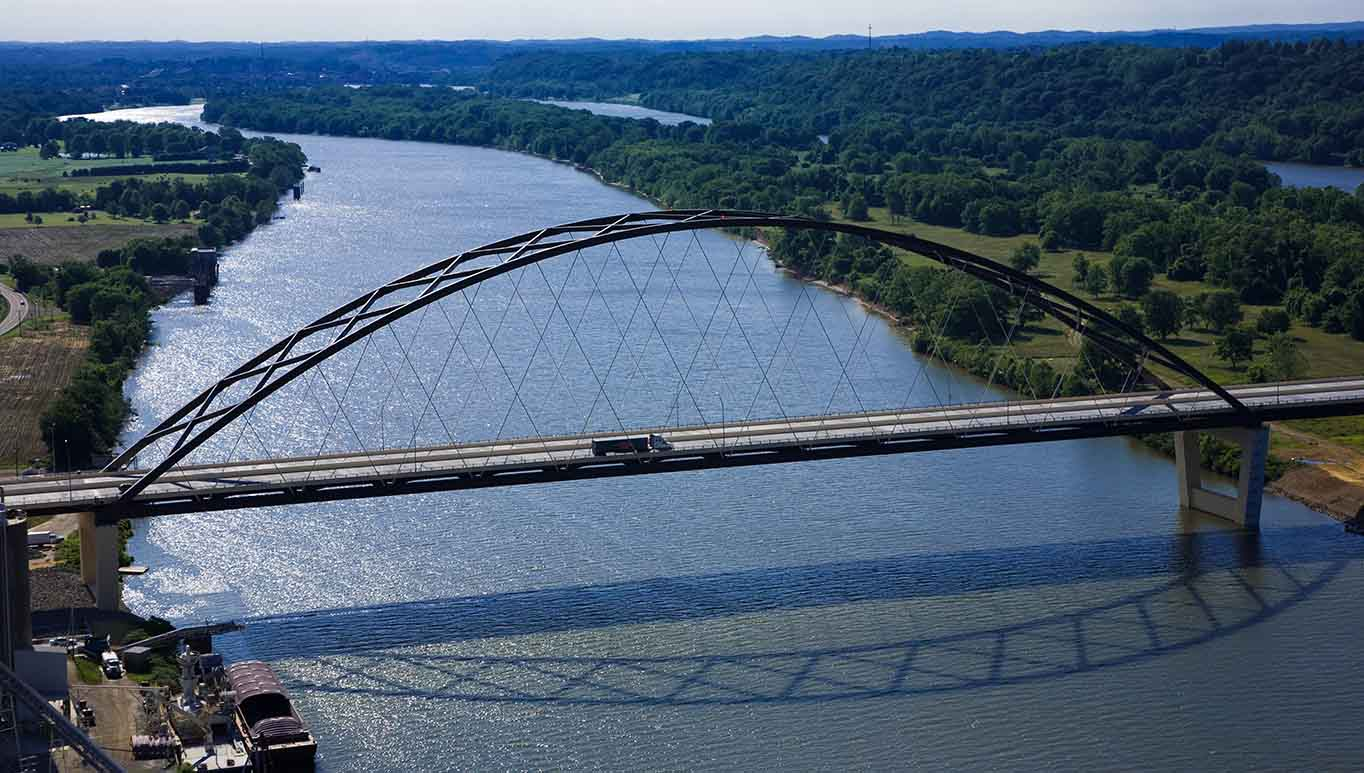
\includegraphics[trim={0 0 0 0},clip, width=0.9\textwidth]{overleaf/Pictures/Blennerhassett_2_1.jpg}
    \caption{Main span (adapted from \cite{Blennerhassett_2})}
    \label{fig:Blennerhassett_1}
\end{subfigure}%
\caption{Blennerhassett Island Bridge}
\label{fig:Blennerhassetts}
\end{figure}

The bridge deck is \SI{30.6}{m} wide giving room for two roadways supporting three lanes.
While a composite deck was chosen for the approach spans, a floating deck system with depth of \SI{0.24}{m} was arranged on the main span. However, also the floating deck relies on composite action with the stringers instead of the tie girder. These stringers are supported on sliding bearings on the floor beams to prevent the introduction of normal forces into the deck. 13 floor beams are arranged at \SI{19.1}{m} spacing spanning the entire width of the deck of \SI{31.4}{m}, where they are fixed into the tie girders. The arch rib and the tie girders are simply supported on the piers with sliding bearings on one side. The hangers are based on the technology for stay cables. At each floor beam, two cables composed of 27 strands are connected to the tie girder. % at angles of \SI{64}{\degree}. 
The resulting hanger spacing on the tie of \SI{19.1}{m} is by this date still the longest. Each cable is protected by a duct and anchored inside the cross section of the arch and the tie to allow for simple installation. The tied-arch was erected in place and two halves. It was closed by jacking at the sliding bearing to overcome the initial offset of \SI{150}{mm} and to introduce the tie tensile action. Further design data relying on the design drawings are presented in \cref{tab:Blennerhassett_design_data}. More details on the cross sections are given in \cref{sec:met_str}.
\begin{table}[H]
    \caption{Design data of the Blennerhassett Island Bridge}
    \label{tab:Blennerhassett_design_data}
    \centering
    \begin{tabular}{cccccc}
    \toprule
    Dead loads & Live loads & Arch geometry & Arch bracing & Hanger pattern & Hanger inclination \\ \midrule
    \SI{210}{kN/m} & \SI{30}{kN/m} & Parabolic & Diamond & Parallel & \SI{64}{\degree}  \\ \bottomrule
    \end{tabular}
\end{table}

\subsection{Other network-tied arch bridges}\label{sec:other_bridges}
For comparative purposes, the design data of a few similar network tied-arch bridges is specified. These are the Amelia Earhart Bridge (Missouri/Kansas), the Wellsburg Bridge (West Virginia/Ohio), the Kentucky Lake Bridge (Kentucky) and the Lake Champlain Bridge (New York/Vermont). The relevant design data is presented in \cref{tab:other_design_data}.

\begin{table}[H]
    \centering    
    \caption{Design data of comparable network tied-arch bridges}
    \label{tab:other_design_data}
    \resizebox{\columnwidth}{!}{%
    \begin{tabular}{llccccl}
\toprule
\textbf{Bridge} & & Amelia Earhart & Wellsburg & Kentucky Lake & Lake Champlain &  \\
& Year & 2012 & 2020 & 2013 & 2010 &  \\ \midrule
\textbf{Dimensions} & Span & 160.6 & 253 & 167.6 & 123 & [m]  \\
& Rise & 26.5 & 39.5 & 32.4 & 24.7 & [m] \\
& Width & 22.1 & 18.1 & 23 & 17.3 & [m] \\
& Width (road) & 21.3 & 14.6 & 18.9 & 9.8 & [m]  \\ \midrule
\textbf{Loads (estimated)} & Dead loads & 145.7 & 160.6 & 138.8 & 104.9 & [kN/m] \\
& Live loads & 19.1 & 14.7 & 19.7 & 11.5 & [kN/m] \\ \midrule
\textbf{Arch} & Geometry & Parabolic & Circular & Parabolic & Circular &  \\
& Bracing & Diamond & Diamond & Cross girder & Diamond &  \\
& Height & 1.45 & 1.88 & 1.22 & 0.91 & [m] \\
& Area & 0.168 & 0.239 & 0.167 & 0.103 & [\SI{}{m^2}] \\ \midrule
\textbf{Tie} & Height & 1.84 & 1.52 & 1.54 & 1.27 & [m] \\
& Area & 0.153 & 0.241 & 0.179 & 0.100 & [\SI{}{m^2}] \\ \midrule
\textbf{Deck} & System & Composite & Floating & Composite & Composite &  \\
& Height & 0.18 & 0.23 & 0.20 & 0.25 & [m] \\ \midrule
\textbf{Hangers} & Pattern & Parallel & Radial & Parallel* & Constant Change &  \\
& Inclination & 61 & $\beta$=30 & 60* & 77-62 & [\degree] \\
& Hangers per set & 14 & 16 & 11 & 16 & [-] \\
& Resistance & 3.3 & 3.8 & 3.0 / 6.0 & 1.8 & [MN] \\ \bottomrule
\end{tabular}

%\begin{tabular}{lccccl}
%\toprule
%\textbf{Bridge} & Amelia Earhart & Wellsburg & Kentucky Lake & %Lake Champlain &  \\
%Year & 2012 & 2020 & 2013 & 2010 &  \\ \midrule
%\textbf{Dimensions} &  &  &  &  &  \\
%Span & 160.6 & 253 & 167.6 & 123 & [m]  \\
%Rise & 26.5 & 39.5 & 32.4 & 24.7 & [m] \\
%Width & 22.1 & 18.1 & 23 & 17.3 & [m] \\
%Width (road) & 21.3 & 14.6 & 18.9 & 9.8 & [m]  \\ \midrule
%\textbf{Loads (estimated)} &  &  &  &  &  \\
%Dead loads & 145.7 & 160.6 & 138.8 & 104.9 & [kN/m] \\
%Live loads & 19.1 & 14.7 & 19.7 & 11.5 & [kN/m] \\ \midrule
%\textbf{Arch} &  &  &  &  &  \\
%Geometry & Parabolic & Circular & Parabolic & Circular &  \\
%Bracing & Diamond & Diamond & Cross girder & Diamond &  \\
%Height & 1.45 & 1.88 & 1.22 & 0.91 & [m] \\
%Area & 0.168 & 0.239 & 0.167 & 0.103 & [\SI{}{m^2}] \\ %\midrule
%\textbf{Tie} &  &  &  &  &  \\
%Height & 1.84 & 1.52 & 1.54 & 1.27 & [m] \\
%Area & 0.153 & 0.241 & 0.179 & 0.100 & [\SI{}{m^2}] \\ %\midrule
%\textbf{Deck} &  &  &  &  &  \\
%System & Composite & Floating & Composite & Composite &  \\
%Height & 0.18 & 0.23 & 0.20 & 0.25 & [m] \\ \midrule
%\textbf{Hangers} &  &  &  &  &  \\
%Pattern & Parallel & Radial & Parallel* & Constant Change &  %\\
%Inclination & 61 & $\beta$=30 & 60* & 77-62 & [\degree] \\
%Hangers per set & 14 & 16 & 11 & 16 & [-] \\
%Resistance & 3.3 & 3.8 & 3.0 / 6.0 & 1.8 & [MN] \\ \bottomrule
%\end{tabular}%
    }
\end{table}

\newpage
\section{Structural model} \label{sec:met_str}
A defining feature of the Blennerhassett Island Bridge is the floating deck. It is responsible for the majority of the structure's weight and is the live loading application point. It is supported only at the 13 floor beams and acts almost structurally independent resembling a bridge by itself. Compared to a composite deck, it causes a certain inefficiency in material use and the additional arrangement of many bearings. On the other hand, it allows for a future replacement of the deck and simplifies the investigation of the flow of forces. It carries the loads over a span of nearly \SI{20}{m} to the adjacent floor beams. There, the forces are carried by the respective hanger pair and partially by the tie girder. This feature allows for a separation of the behaviour of the remaining network arch from the deck. As it is not the objective of this Thesis to investigate and optimise the deck system, it is not further considered. According to Smit, the behaviour of the two planes of the arch can be considered decoupled from each other \cite{Smit}. Therefore, the network arch's behaviour is analysed in a single arch plane considering the arch rib, the tie girder and the hangers. In the design drawings, the structure is further divided into segments for the arch and the tie. Each of these segments is verified independently in the design verifications. The respective segmentation, shown along with the bridge in \cref{fig:Blennerhassett2_a} and \cref{fig:Blennerhassett2_b}, is also used for the investigation in this Thesis.

\begin{figure}[H]
\centering
\begin{subfigure}{0.5\textwidth}
    \centering
    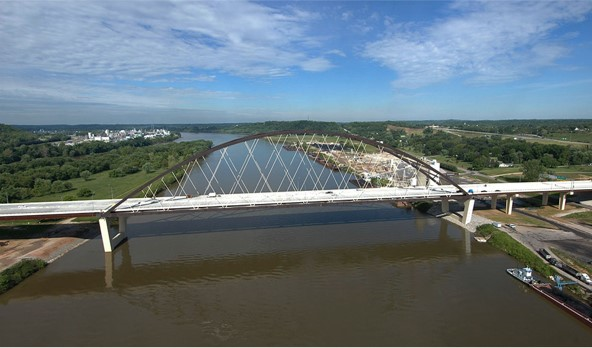
\includegraphics[width=0.9\textwidth]{overleaf/Pictures/Blennerhassett_2.jpg}
    \caption{Built structure}
    \label{fig:Blennerhassett2_a}
\end{subfigure}%
\begin{subfigure}{.5\textwidth}
    \centering
    \vspace*{0.67cm}
    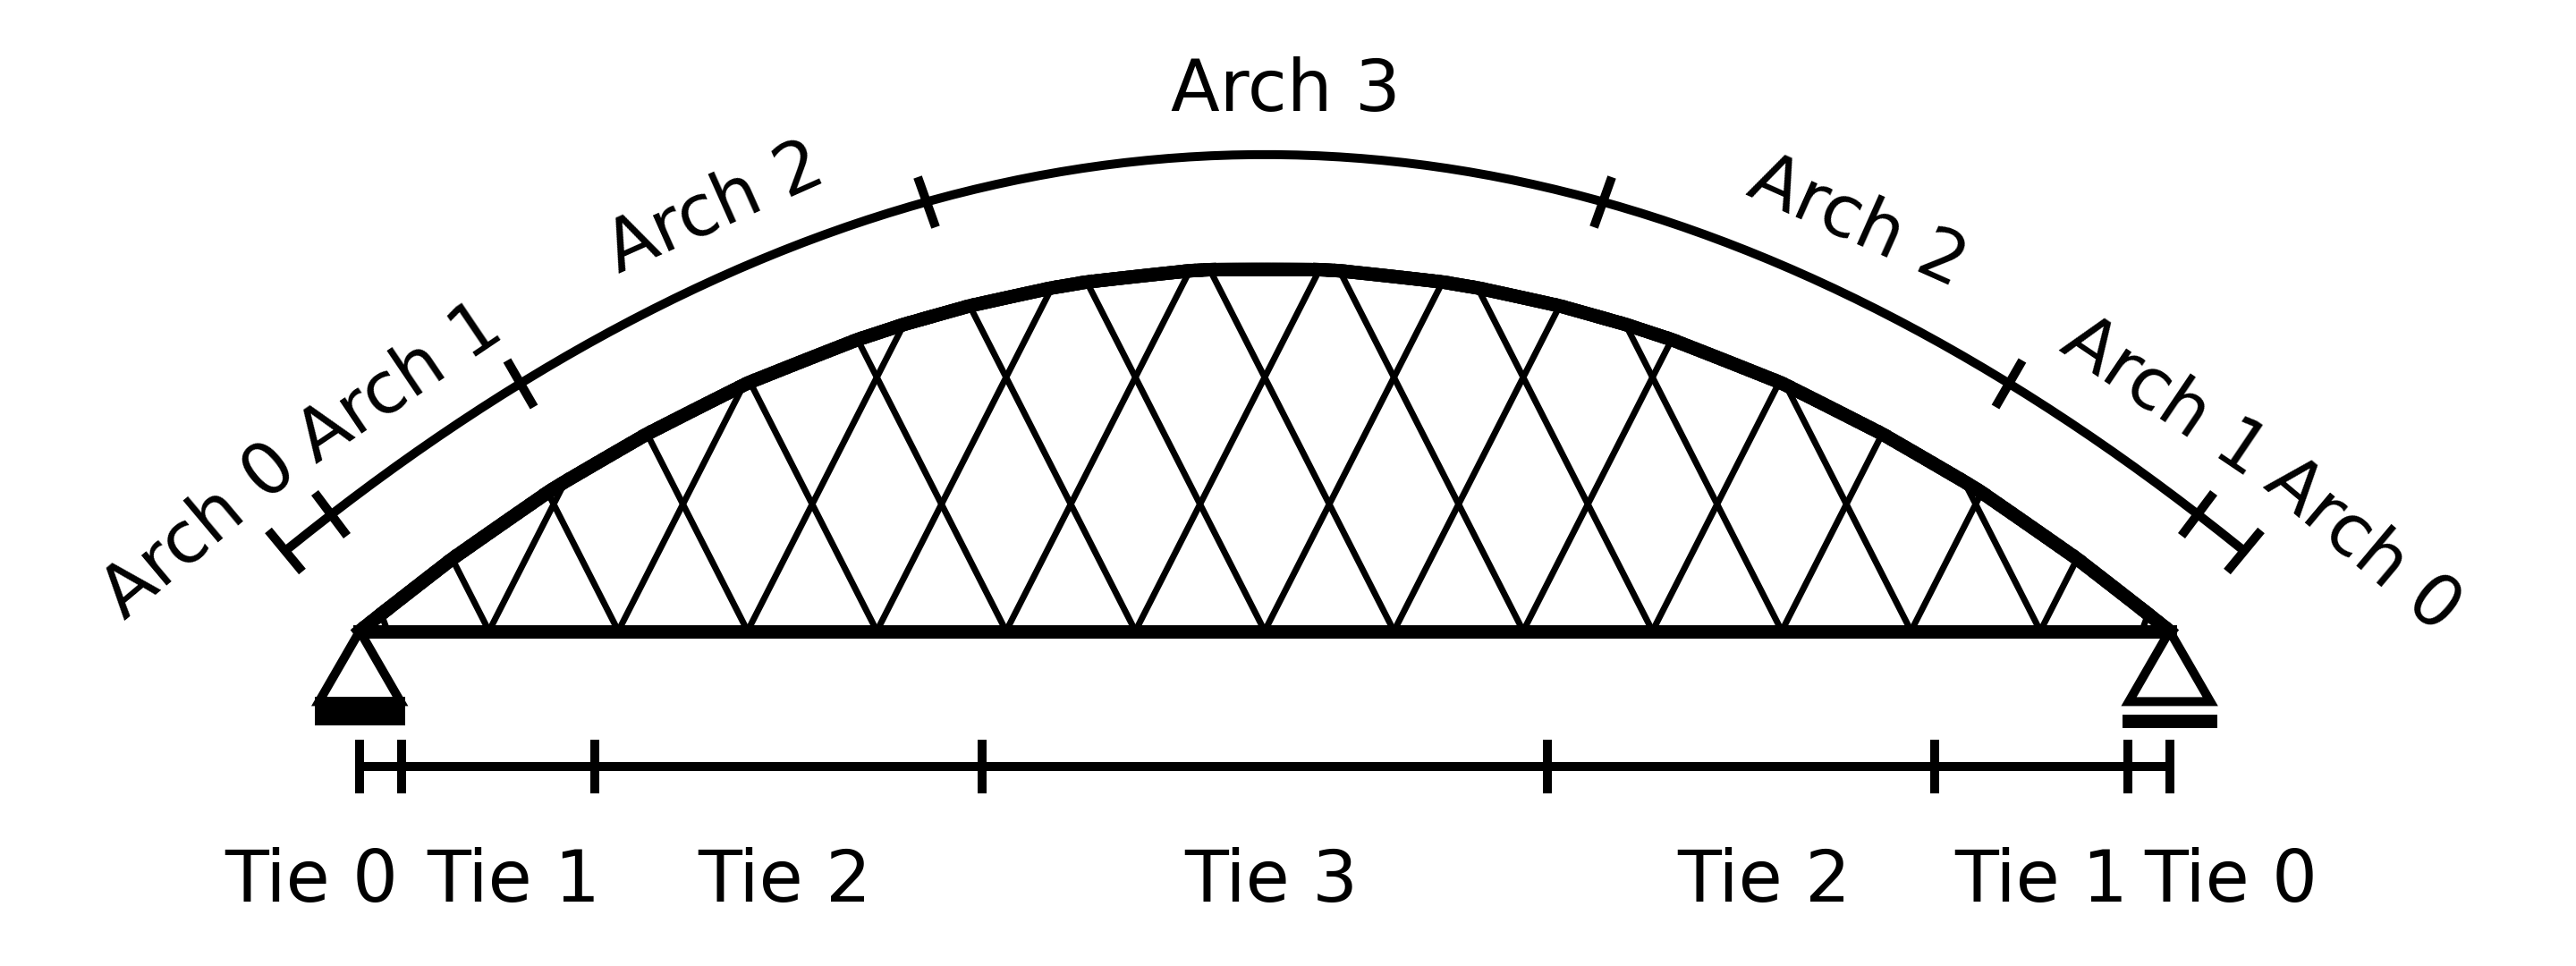
\includegraphics[width=0.9\textwidth]{illustrations/figures/segments.png}
    \vspace*{0.67cm}
    \caption{Structural model and segments}
    \label{fig:Blennerhassett2_b}
\end{subfigure}
\caption{Blennerhassett Island Bridge}
\label{fig:Blennerhassett2}
\end{figure}

Both the arch and the tie girder feature a box cross-section with a width of \SI{1.2}{m}. The arch is \SI{1.7}{m} high and offers similar bending resistances around both axes. Additionally, it is reinforced by a web stiffener to prevent local buckling. The cross section of the tie girder is \SI{2.2}{m} high and offers more resistance for longitudinal than transverse bending moments. The arch rib and the tie girder feature a stronger cross-section in the knuckle region, where the highest internal force effects are expected. The segments Arch 0 and Tie 0 form the knuckle and are assigned the strongest cross-sections, with resistances roughly 50\% higher than in the field. They are not subject to the optimisation in this Thesis as they cannot accurately be dimensioned as beam elements. The next segments, Arch 1 and Tie 1, also have a slightly enhanced cross-section with thicker plates. The remaining segments in the field feature identical cross-sections for the tie girder and the arch rib respectively. They are considered the characteristic cross-sections and are shown in \cref{fig:cs_arch} and \cref{fig:cs_tie}. All cables have identical cross-sections with 27 high-strength strands of \SI{140}{mm^2}. The respective lengths range from \SI{11}{m} to \SI{59}{m}. The corresponding cross-section including its tube is shown in \cref{fig:cs_cable}. The most important properties of the characteristic cross sections are specified in \cref{tab:cs_properties}. More detailed specifications are found in \cref{app:cross_sections}.

\begin{figure}[H]
\centering
\begin{subfigure}{0.33\textwidth}
    \centering
    \vspace*{0.68cm}
    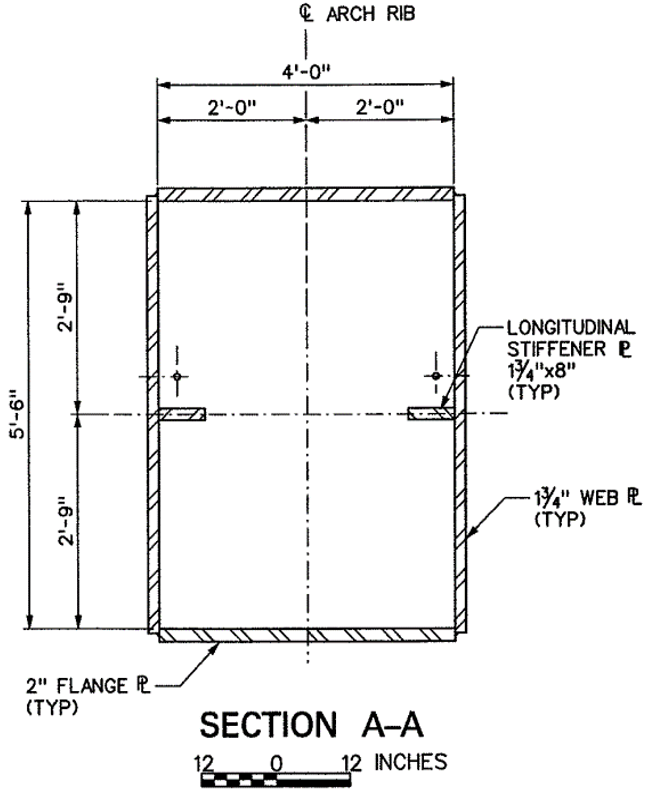
\includegraphics[width=0.8\textwidth]{overleaf/Appendix/Pictures/arch_3.PNG}
    \vspace*{0.68cm}
    \caption{Arch rib}
    \label{fig:cs_arch}
\end{subfigure}%
\begin{subfigure}{.33\textwidth}
    \centering
    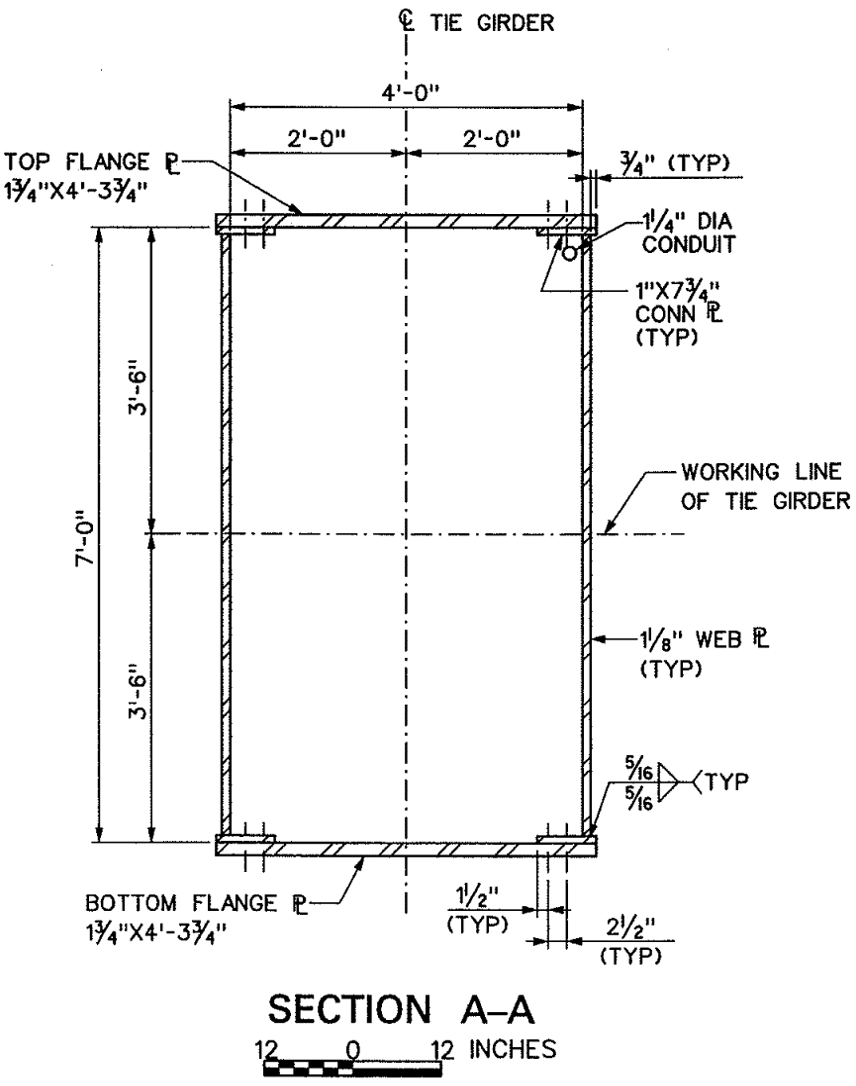
\includegraphics[width=\textwidth]{overleaf/Appendix/Pictures/tie_3.PNG}
    \caption{Tie girder}
    \label{fig:cs_tie}
\end{subfigure}%
\begin{subfigure}{.33\textwidth}
    \centering
    \vspace*{1.35cm}
    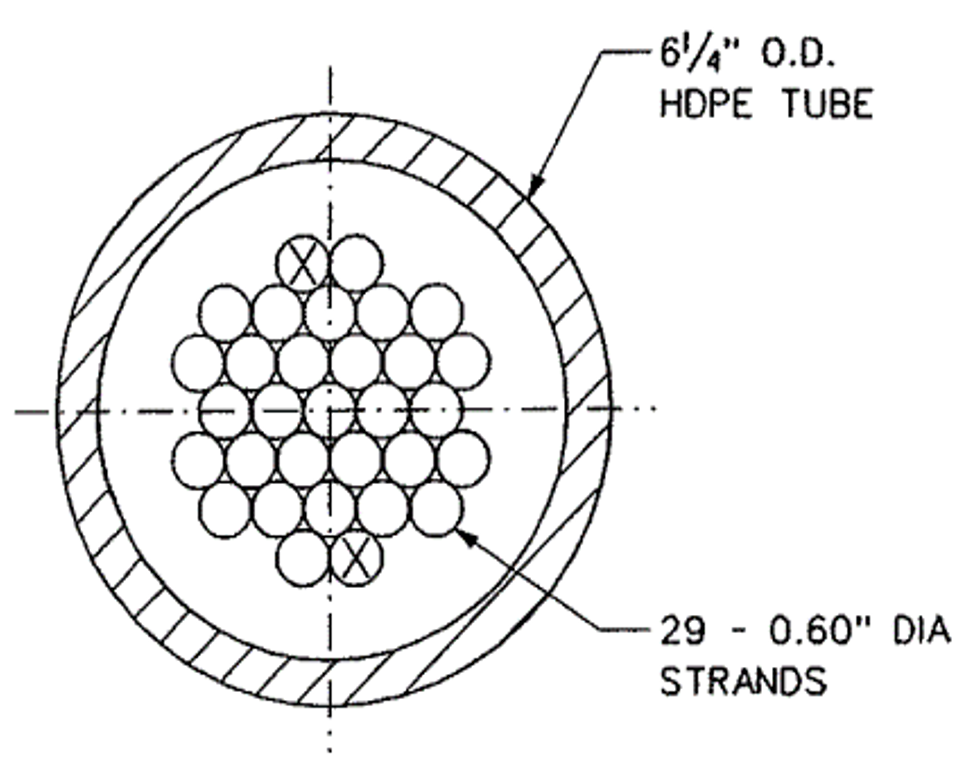
\includegraphics[width=0.9\textwidth]{overleaf/Appendix/Pictures/cable_3.PNG}
    \vspace*{1.35cm}
    \caption{Cable}
    \label{fig:cs_cable}
\end{subfigure}\caption{Cross-sections in the field}
\label{fig:cross_sections}
\end{figure}

\begin{table}[H]
    \centering
    \caption{Properties of the field cross-sections}
    \label{tab:cs_properties}
    \begin{tabular}{lccccc}
    \toprule
    Cross-section & $EA$ & $EI$ & $N_{Rd}$ & $M_{Rd,z}$ & $M_{Rd,y}$ \\
                  & [\SI{}{GN}]   & [\SI{}{GNm^2}]   & [\SI{}{MN}]  & [\SI{}{MNm}]  & [\SI{}{MNm}] \\ \midrule
    Arch 2 \& 3 & 61.8 & 28.1 & 82.3 & 50.0 & 42.7 \\
    Tie 2 \& 3  & 53.7 & 42.8 & 100.5 & 76.2 & 45.8 \\
    Cables        & 0.8 &  - & 6.8 & - & - \\ \bottomrule
    \end{tabular}
\end{table}

The arch and the tie are accurately modelled as Bernoulli beam elements, considering their slenderness. The curvature of the arch rib is neglected and modelled by a series of straight elements, as the difference is practically negligible ($r>10\,h$) \cite{MARTI}. On the other hand, secondary effects cannot always be neglected for the hangers because of their low bending stiffness. However, a brief investigation, given in \cref{Appendix_A_Hangers}, shows that above \SI{100}{MPa} these effects are irrelevant. Therefore, the hangers are modelled as beam elements with rotational end releases and their self-weight is neglected. Hence, they only carry normal forces. Additionally, two web plates connecting the tie girder and the arch rib in the knuckle region are arranged to obtain a more accurate representation of this detail. Each web plate has a cross section of \SI{6.3}{cm} x \SI{1.07}{m} and is arranged \SI{4.1}{m} for the idealised node at an angle of 80\degree. The arrangement of the web plates is illustrated in \cref{fig:knuckle_region}.


\begin{figure}[H]
    \centering
    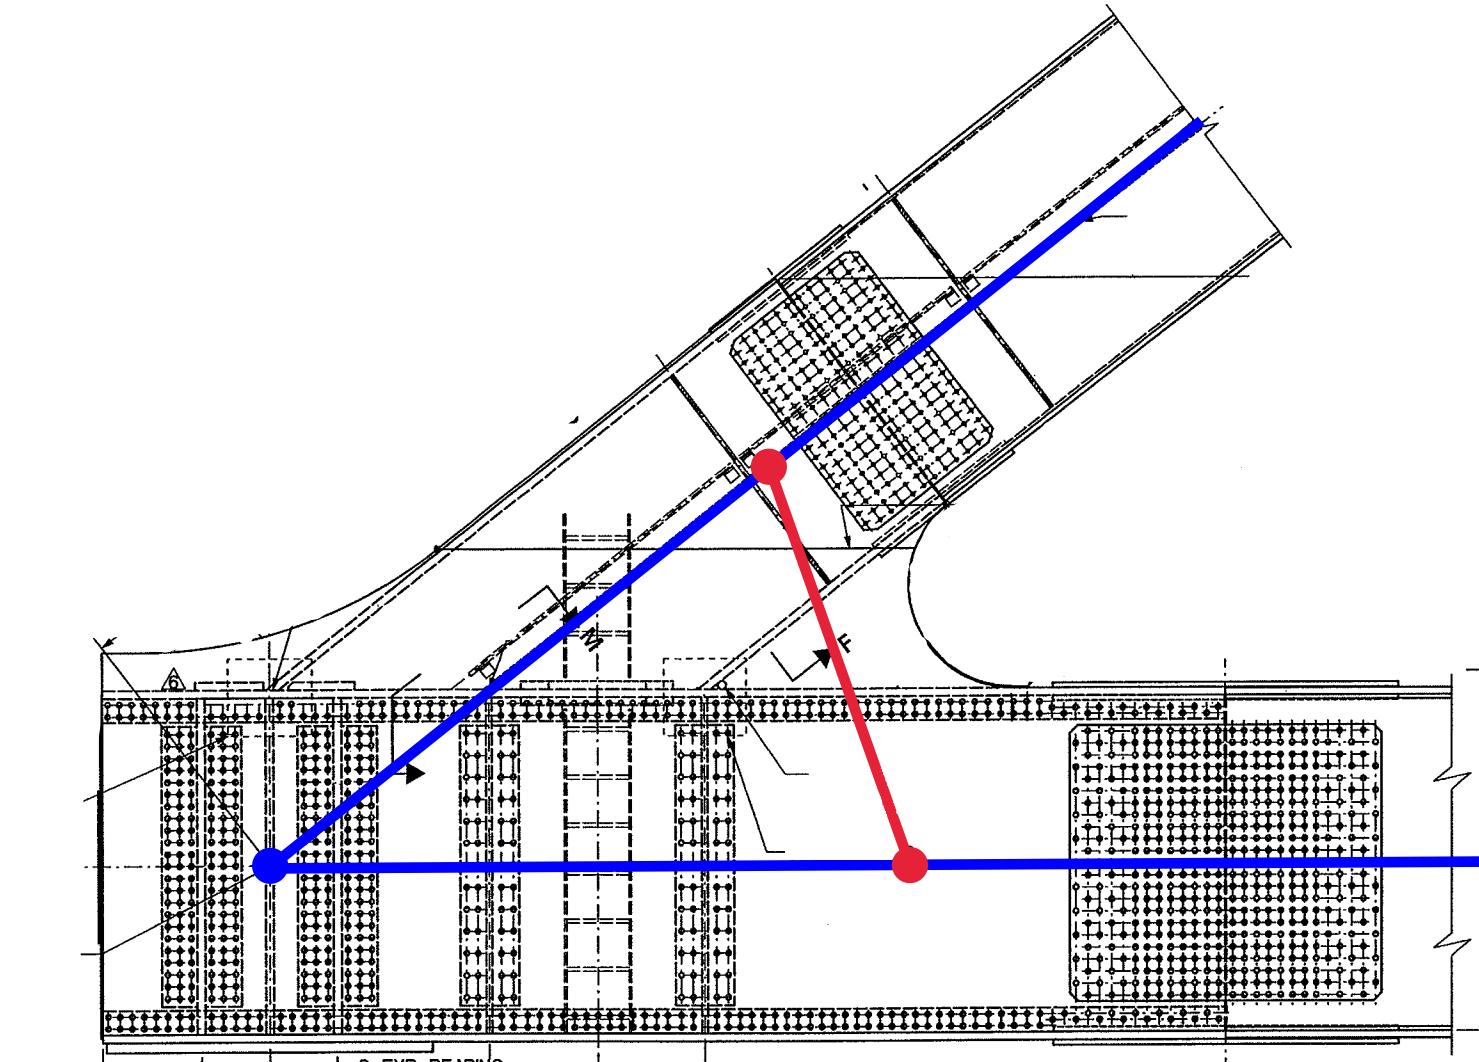
\includegraphics[width=0.42\textwidth]{overleaf/Pictures/Knuckle region.png}
    \caption{Plan and structural model of the knuckle region}
    \label{fig:knuckle_region}
\end{figure}

The structure is analysed in the framework of two-dimensional and linear elastic beam statics. For the structural analysis, a python package written by the author in an earlier project is used. It is verified with the Sofistik model of a parallel Master Thesis in \cref{app:model_verification}. The structure is first analysed using different simplified models to judge the impact on the resulting internal force effects. In the first simplistic model, the field cross-sections are used everywhere and also no web member is considered. In a second model, the previously described web plates are introduced. Ultimately, the actual cross-sections are assigned to the arch and the tie in a third model. The most important elastic effects under dead loads for each component are compared in \cref{fig:model_comparison}. For the hangers, only the hanger set inclined towards the right side is shown.

\begin{figure}[H]
    \centering
    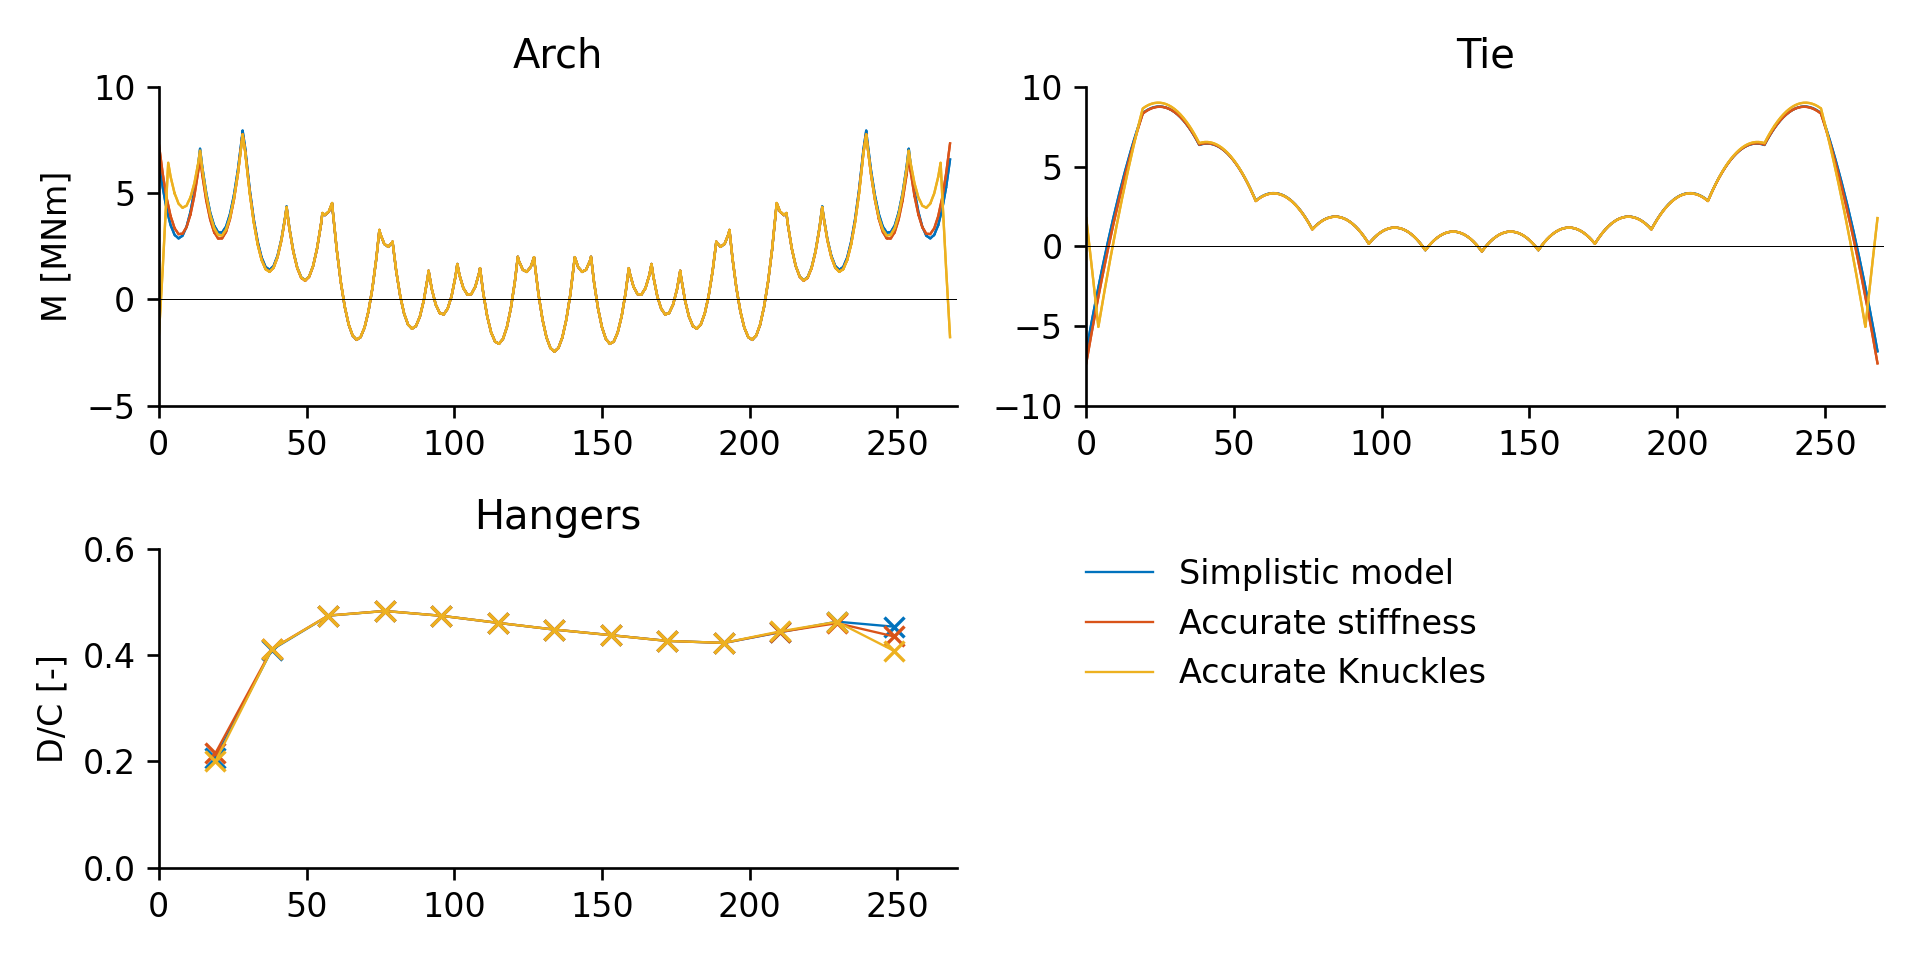
\includegraphics[width=\textwidth]{calculations/model comparison/dead_loading.png}
    \caption{Comparison of the elastic responses under dead loading for different models}
    \label{fig:model_comparison}
\end{figure}

The differences among the models are negligible. Only for the shortest hangers the demand slightly decreases in the accurate models. The stiffnesses in the knuckle region, therefore, do not have significant impacts on the flow of forces. Nevertheless, a model featuring accurate stiffnesses and including the web plate in the knuckle region is used for the investigation. The accurate stiffness is considered to remain consistent with the increased cross-sectional resistances considered for the design verifications. On the other hand, the web plates facilitate the calculation of the thrust line for the permanent effects, as presented in \cref{sec:met_arch}.

\newpage
\section{Load cases} \label{sec:met_loads}
The load cases relevant to this investigation are the dead loading (DL), the live loading (LL) and the wind loading (WS). The dead loading is further subdivided into the weight of the structural components and non-structural attachments (DC) and the weight of the future wearing surfaces and utilities (DW).

\subsection{Dead loading}
The dead loads for the Blennerhassett Island Bridge are derived from the estimated bridge quantities from the design drawings. The detailed derivation is given in \cref{app:weight} and the final results are presented in \cref{tab:dead_loads}. The weight of the arch and the tie girder are distributed as a uniform load along the respective elements. A particularly detailed weight distribution by assigning more weight to the stronger cross-sections near the knuckle is disregarded for. Also the weight of the arch bracing is distributed along the entire arch for simplicity. The deck weight and its non-structural components make up for the main contribution to the dead loading. Also included is the weight of the floor beams, the tie bracing and the stringers. The weight of the deck is applied as a concentrated force at the locations of the floor beams. The weight of the hangers is relatively small and is neglected to facilitate some of the used optimisation methods. An illustration of the dead loading is shown in \cref{fig:dead_loads}.

\begin{table}[H]
    \centering
    \caption{Weights of the structural and non-structural components}
    \label{tab:dead_loads}
    \begin{tabular}{lcccc}
        \toprule
        Component & Arch & Tie & Deck & Utilities \\ \midrule
        Weight & \SI{29.8}{kN/m} & \SI{26.4}{kN/m} & \SI{115.3}{kN/m} & \SI{35.1}{kN/m} \\ \bottomrule
    \end{tabular}
\end{table}

\begin{figure}[H]
    \centering
    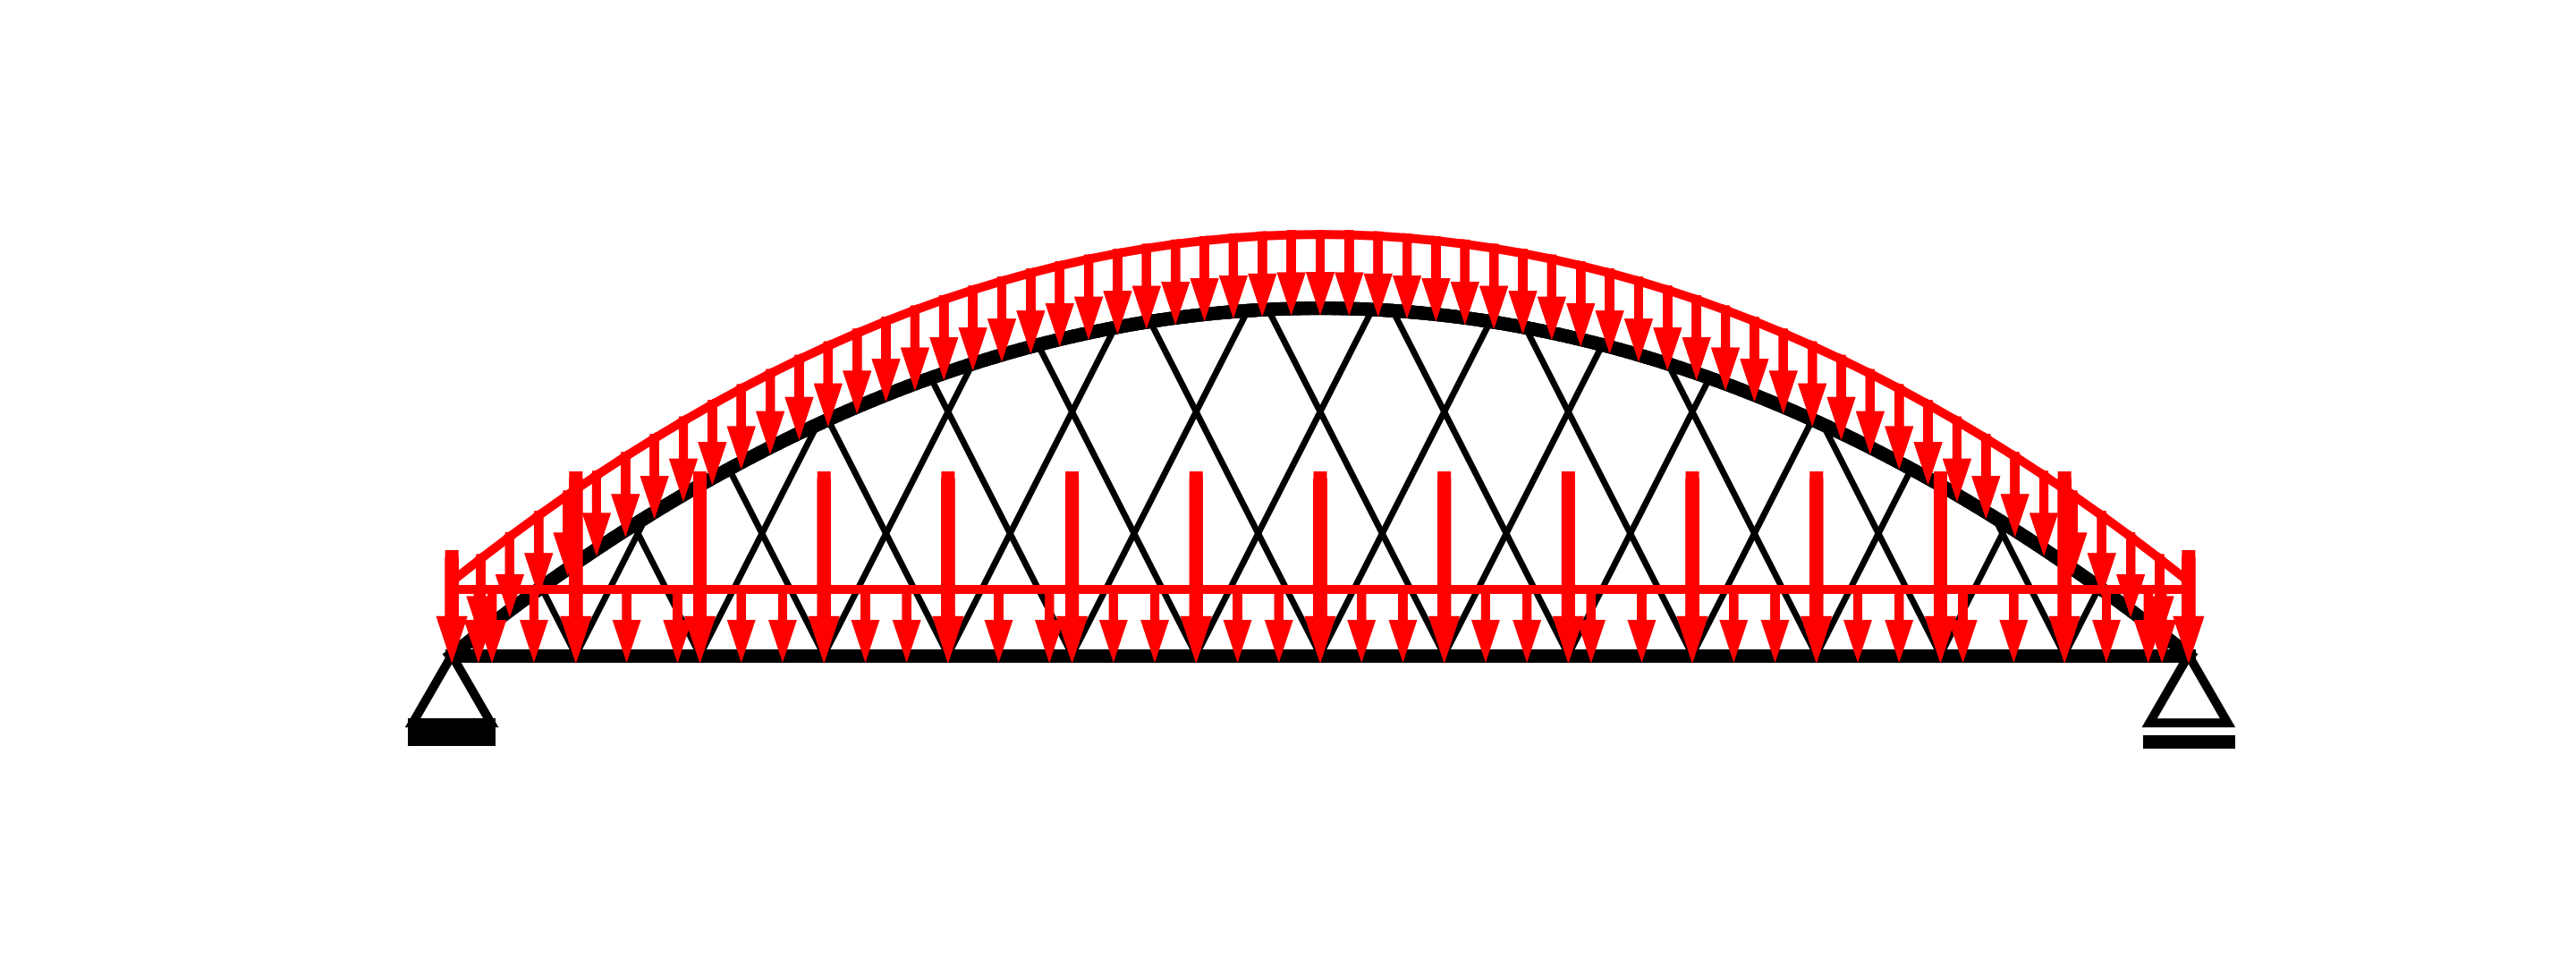
\includegraphics[trim={0 0.8cm 0 0.8cm},clip,
    width=0.8\textwidth]{illustrations/figures/permanent loads.png}
    \caption{Dead loading in the structural model}
    \label{fig:dead_loads}
\end{figure}

\subsection{Live loading} \label{sec:met_loads_live}
The load case of live loading is taken into account according to the AASHTO Bridge Design Specifications (1998) \cite{AASHTO}. It is a combination of two separate components: A lane-wise distributed load is applied along the entire or partial length of the bridge, and concentrated truck loads are applied at a single longitudinal point. Both loads are factored by a multiple presence factor depending on how many lanes are loaded. In a detailed calculation in \cref{Appendix_Liveloading}, six loaded lanes were found to cause the highest load in the considered arch plane for the strength limit state. This conclusion also applies to the truck loads, which is increased by a dynamic multiplier. An overview of the design loads is given in \cref{tab:live_load_overview}. 

\begin{table}[H]
\centering
\caption{Overview of the live loading}
\label{tab:live_load_overview}
\begin{tabular}{cccccc}
\begin{tabular}[c]{@{}c@{}}Design\\ lane load\end{tabular} & \begin{tabular}[c]{@{}c@{}}Design\\ truck weight\end{tabular} & \begin{tabular}[c]{@{}c@{}}Lane\\ multiplier\end{tabular} & \begin{tabular}[c]{@{}c@{}}Dynamic\\ multiplier\end{tabular} & \begin{tabular}[c]{@{}c@{}}Distributed\\ design load\end{tabular} & \begin{tabular}[c]{@{}c@{}}Concentrated\\ design load\end{tabular} \\ \hline
\SI{9.3}{kN/m} & \SI{325}{kN} & \SI{2.46}{} & \SI{1.33}{} & \SI{23.0}{kN/m} & \SI{1063}{kN}
\end{tabular}
\end{table}


The live loads are applied on the deck, which is not part of the structural model. Therefore, the live loads act as concentrated forces on the supporting floor beams as illustrated in \cref{fig:Live_load_1} for the fully loaded deck. The concentrated forces are applied individually to find the worst arrangement of the live loads. For each point of interest in the model, the partially distributed lane load and the concentrated truck load are combined to produce maximum effects. The concentrated force is only applied at one floor beam exclusively, as shown in \cref{fig:Live_load_2}. 

%It yields a range of possible effects for each point on the structural elements. The Blennerhassett Island Bridge's resulting ranges are presented in [], where the ranges of the concentrated load and the distributed loads are also shown individually. These results agree well with the effects specified on the design drawings.\bigskip

\begin{figure}[H]
\centering
\begin{subfigure}{0.5\textwidth}
    \centering
    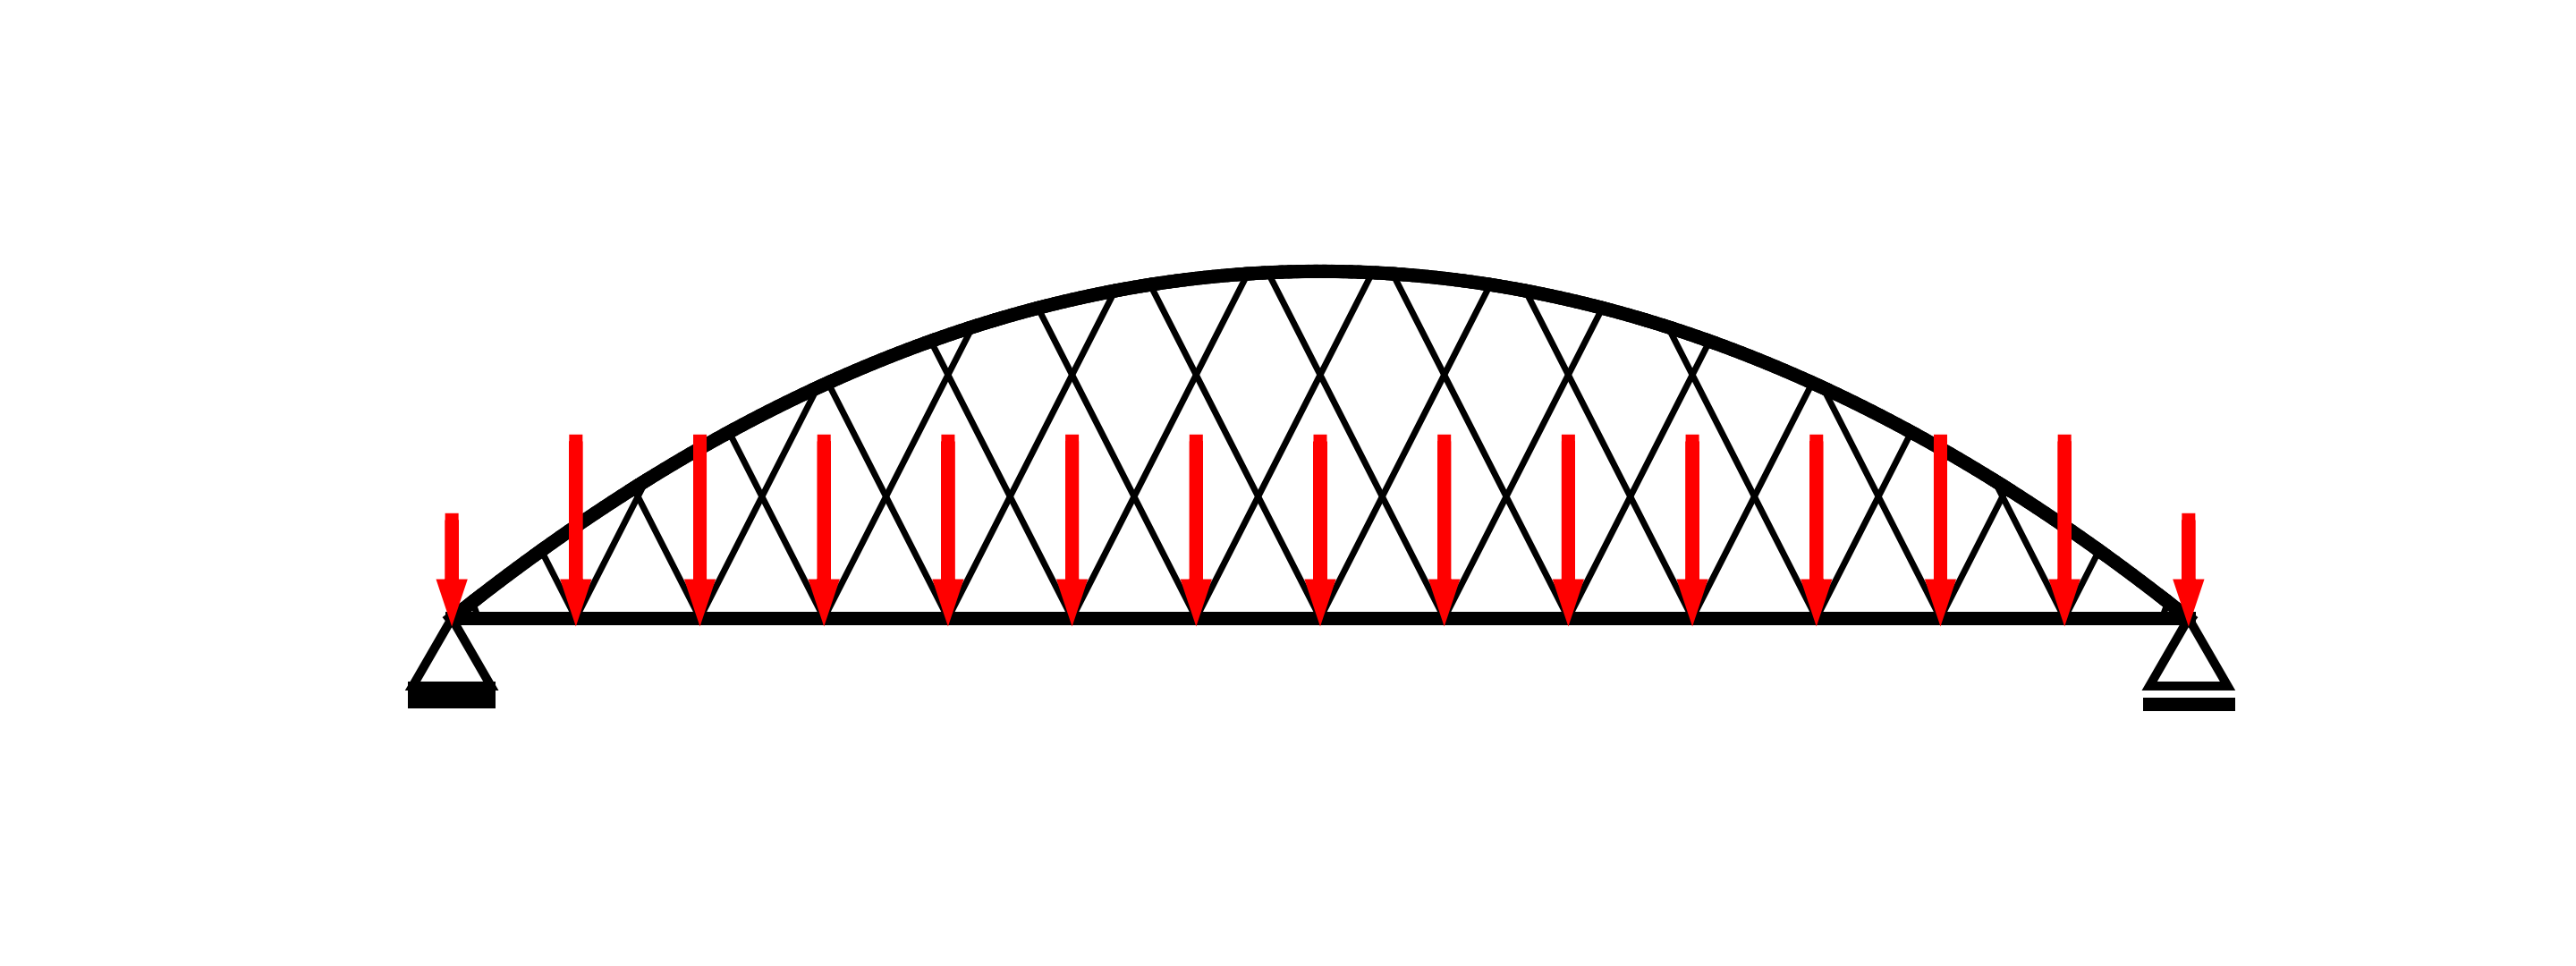
\includegraphics[trim={0 0.8cm 0 0.8cm},clip, width=0.9\textwidth]{illustrations/figures/distributed live loads.png}
    \caption{Distributed live loads}
    \label{fig:Live_load_1}
\end{subfigure}%
\begin{subfigure}{.5\textwidth}
    \centering
    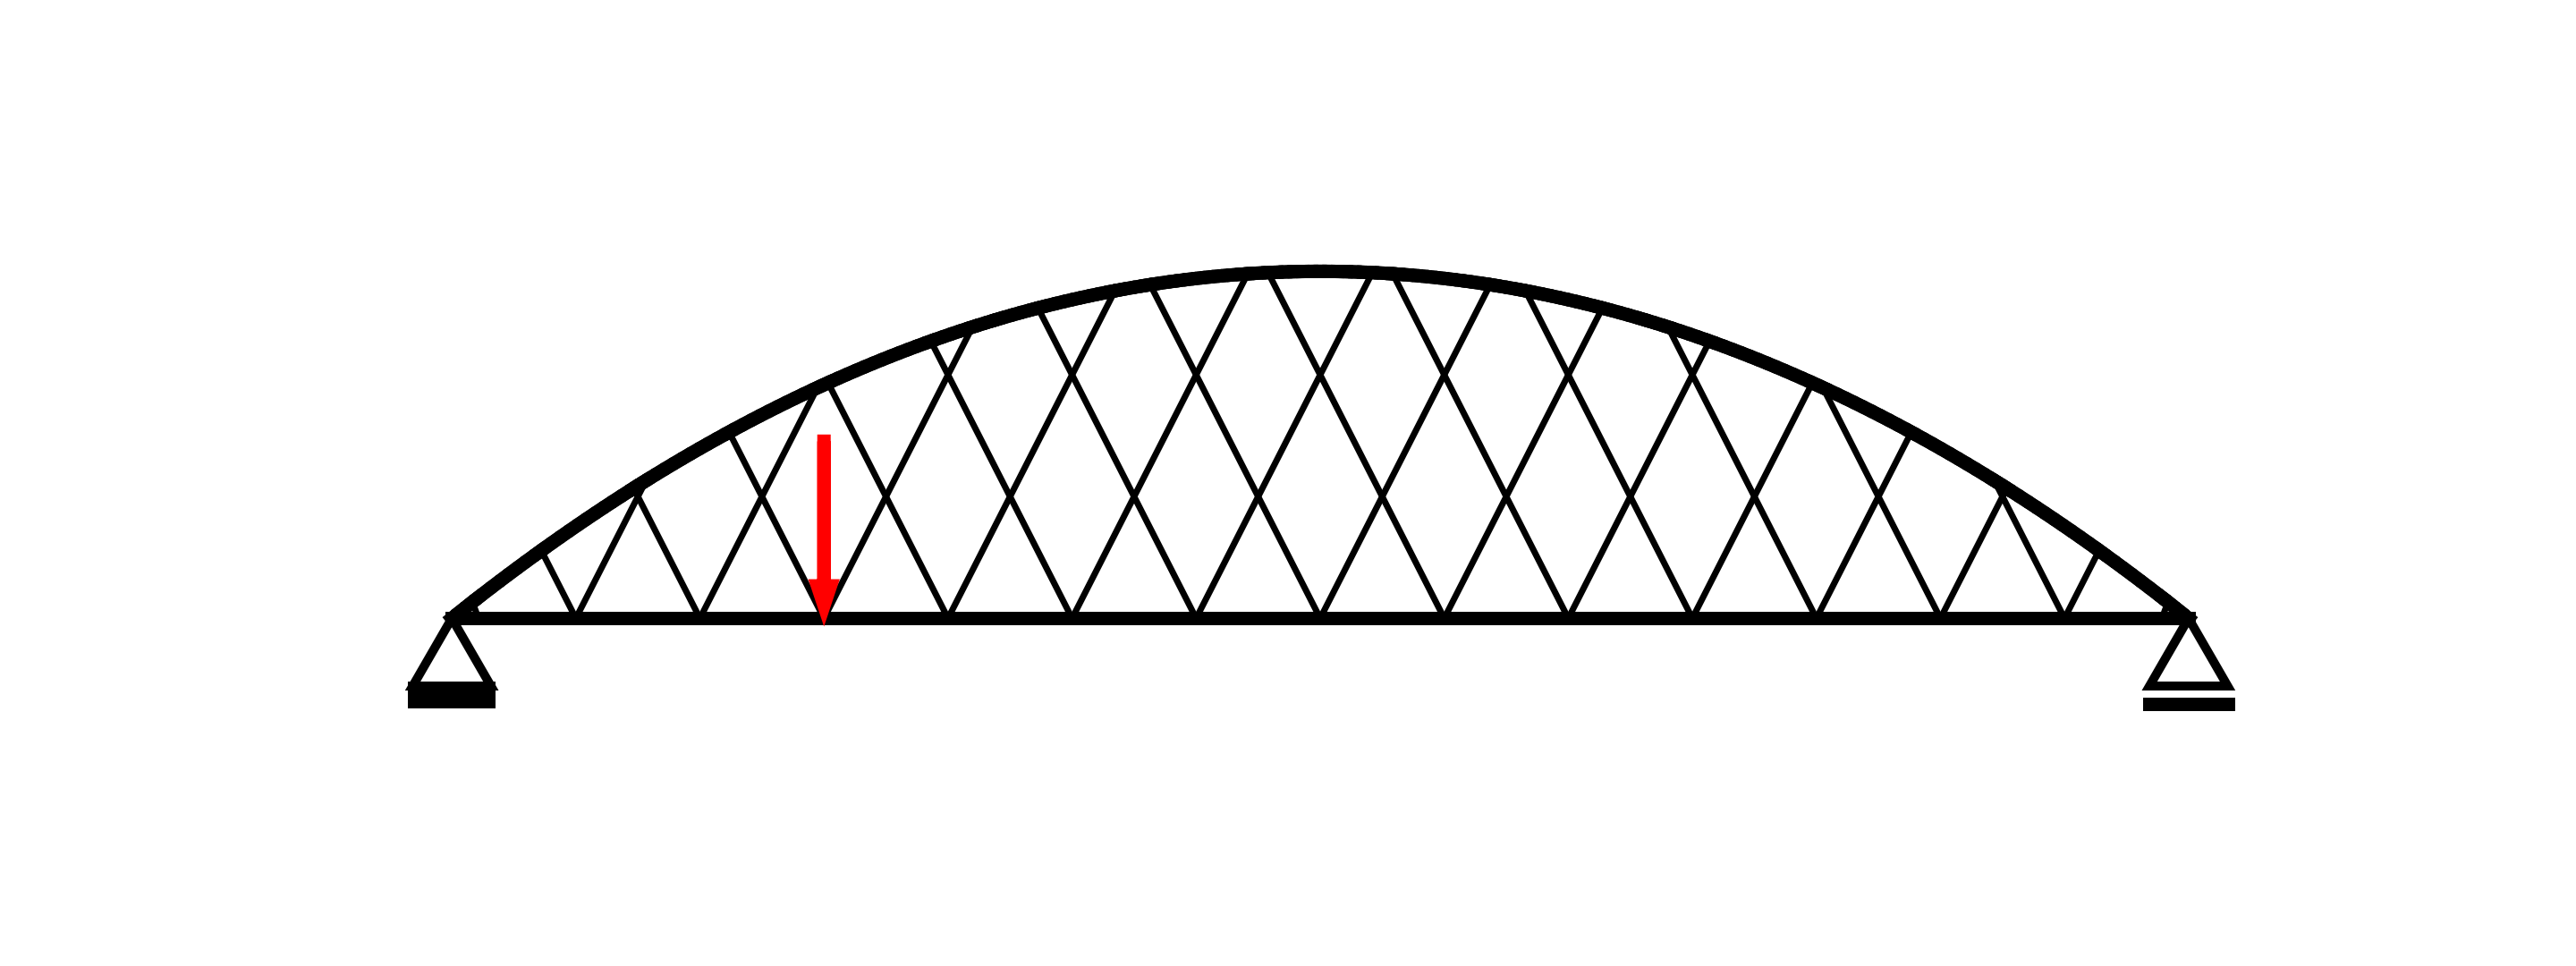
\includegraphics[trim={0 0.8cm 0 0.8cm},clip, width=0.9\textwidth]{illustrations/figures/concentrated live loads.png}
    \caption{Concentrated live loads}
    \label{fig:Live_load_2}
\end{subfigure}
\caption{Live loading in the structural model}
\label{fig:Live_load}
\end{figure}

For the extreme events of cable loss and cable replacement, special circumstances apply to the traffic conditions. For cable loss, it is assumed that only the actually marked lanes are loaded. For cable replacement, one lane is shifted away from the replaced hanger. The determining live load arrangement is calculated and illustrated in \cref{Appendx_A_Live_loading_2}. The resulting loads are given in \cref{tab:live_load_extreme}. For the event of tie fracture, the same live loading as in the strength limit states is applied.

\begin{table}[H]
\centering
\caption{Live loads for extreme events}
\label{tab:live_load_extreme}
\begin{tabular}{lcc}
\hline
Extreme event     & Distributed live load & Concentrated live load \\ \hline
Cable loss  & \SI{14.2}{kN/m} & \SI{660}{kN} \\
Cable replacement & \SI{18.8}{kN/m} & \SI{874}{kN} \\ \hline
\end{tabular}
\end{table}


For the fatigue limit state, the loading according to the PTI specifications is used \cite{PTI}. It consists of a single design truck without taking into account the dynamic multiplier. The resulting force, which is derived in the \cref{Appendx_A_Live_loading_2}, is equal to \SI{296}{kN}.


\subsection{Wind loading}
The load case of wind loading is not calculated in this investigation as the loads are particular to a specific design and require a 3-dimensional model and a very detailed investigation. However, the effects specified on the design drawings, shown in the \cref{app:design_verifications}, are taken to allow for integral design verifications. The respective characteristic internal force effects under wind loading are shown for each segment in \cref{tab:effects_wind_load}.

\begin{table}[H] 
\caption{Effects of wind loading per segment}
\label{tab:effects_wind_load}
\centering
\begin{tabular}{lccc}
\hline
Segment & Normal force & Moment-y & Moment-z \\
 & [MN]   & [MNm] & [MNm] \\ \hline
Arch 1 & -7.8 & -0.67 & 10.7\\
Arch 2 & -4.1 & -0.53 & 2.6\\
Arch 3 & -3.9 & 0.12 & 0.11\\
Tie 1 & 7.0 & -1.1 & 5.9\\
Tie 2 & 6.2 & 0.40 & 0.43\\
Tie 3 & 5.3 & 0.70 & 0.79\\
Hangers & 0.48 & - & - \\ \hline
\end{tabular}
\end{table}


%In [] it is mentioned, that the deciding load case for the design of the Blennerhassett Island Bridge is the accidental tie fracture event. It assumes that one of the flanges or the webs of the tie ruptures, which causes immense stresses and strains on the remaining components and also changes the flow of forces. The investigation of this load case lies outside of the scope of this Thesis. Nevertheless, it is indirectly considered in the objective function, which is introduced in Sec. [].

\newpage
\section{Self-equilibrium stress state} \label{sec:met_seq}
% Permanent state
In an n-times statically indeterminate structure, there are n supernumerary forces or moments. These forces are present in the initial configuration even without any applied loads and cause residual stresses. In the case of a network tied-arch bridge, these residual stresses can be controlled during the construction by prestressing the hangers and applying forces to the arch rib and the tie girder when the two are closed and locked. The created self stress state is in equilibrium with itself and will underlie all following load cases. Therefore, it can counteract the effects expected in the strength limit states and simplify the design verifications. Any set of supernumerary forces describes this self-equilibrium stress state. For the investigation in this Thesis, the supernumerary forces presented in \cref{fig:super_forces} are used. Besides the normal forces in the hangers, the moments between the arch and the tie and the horizontal force at the right knuckle are part of the supernumerary set.

\begin{figure}[H]
    \centering
    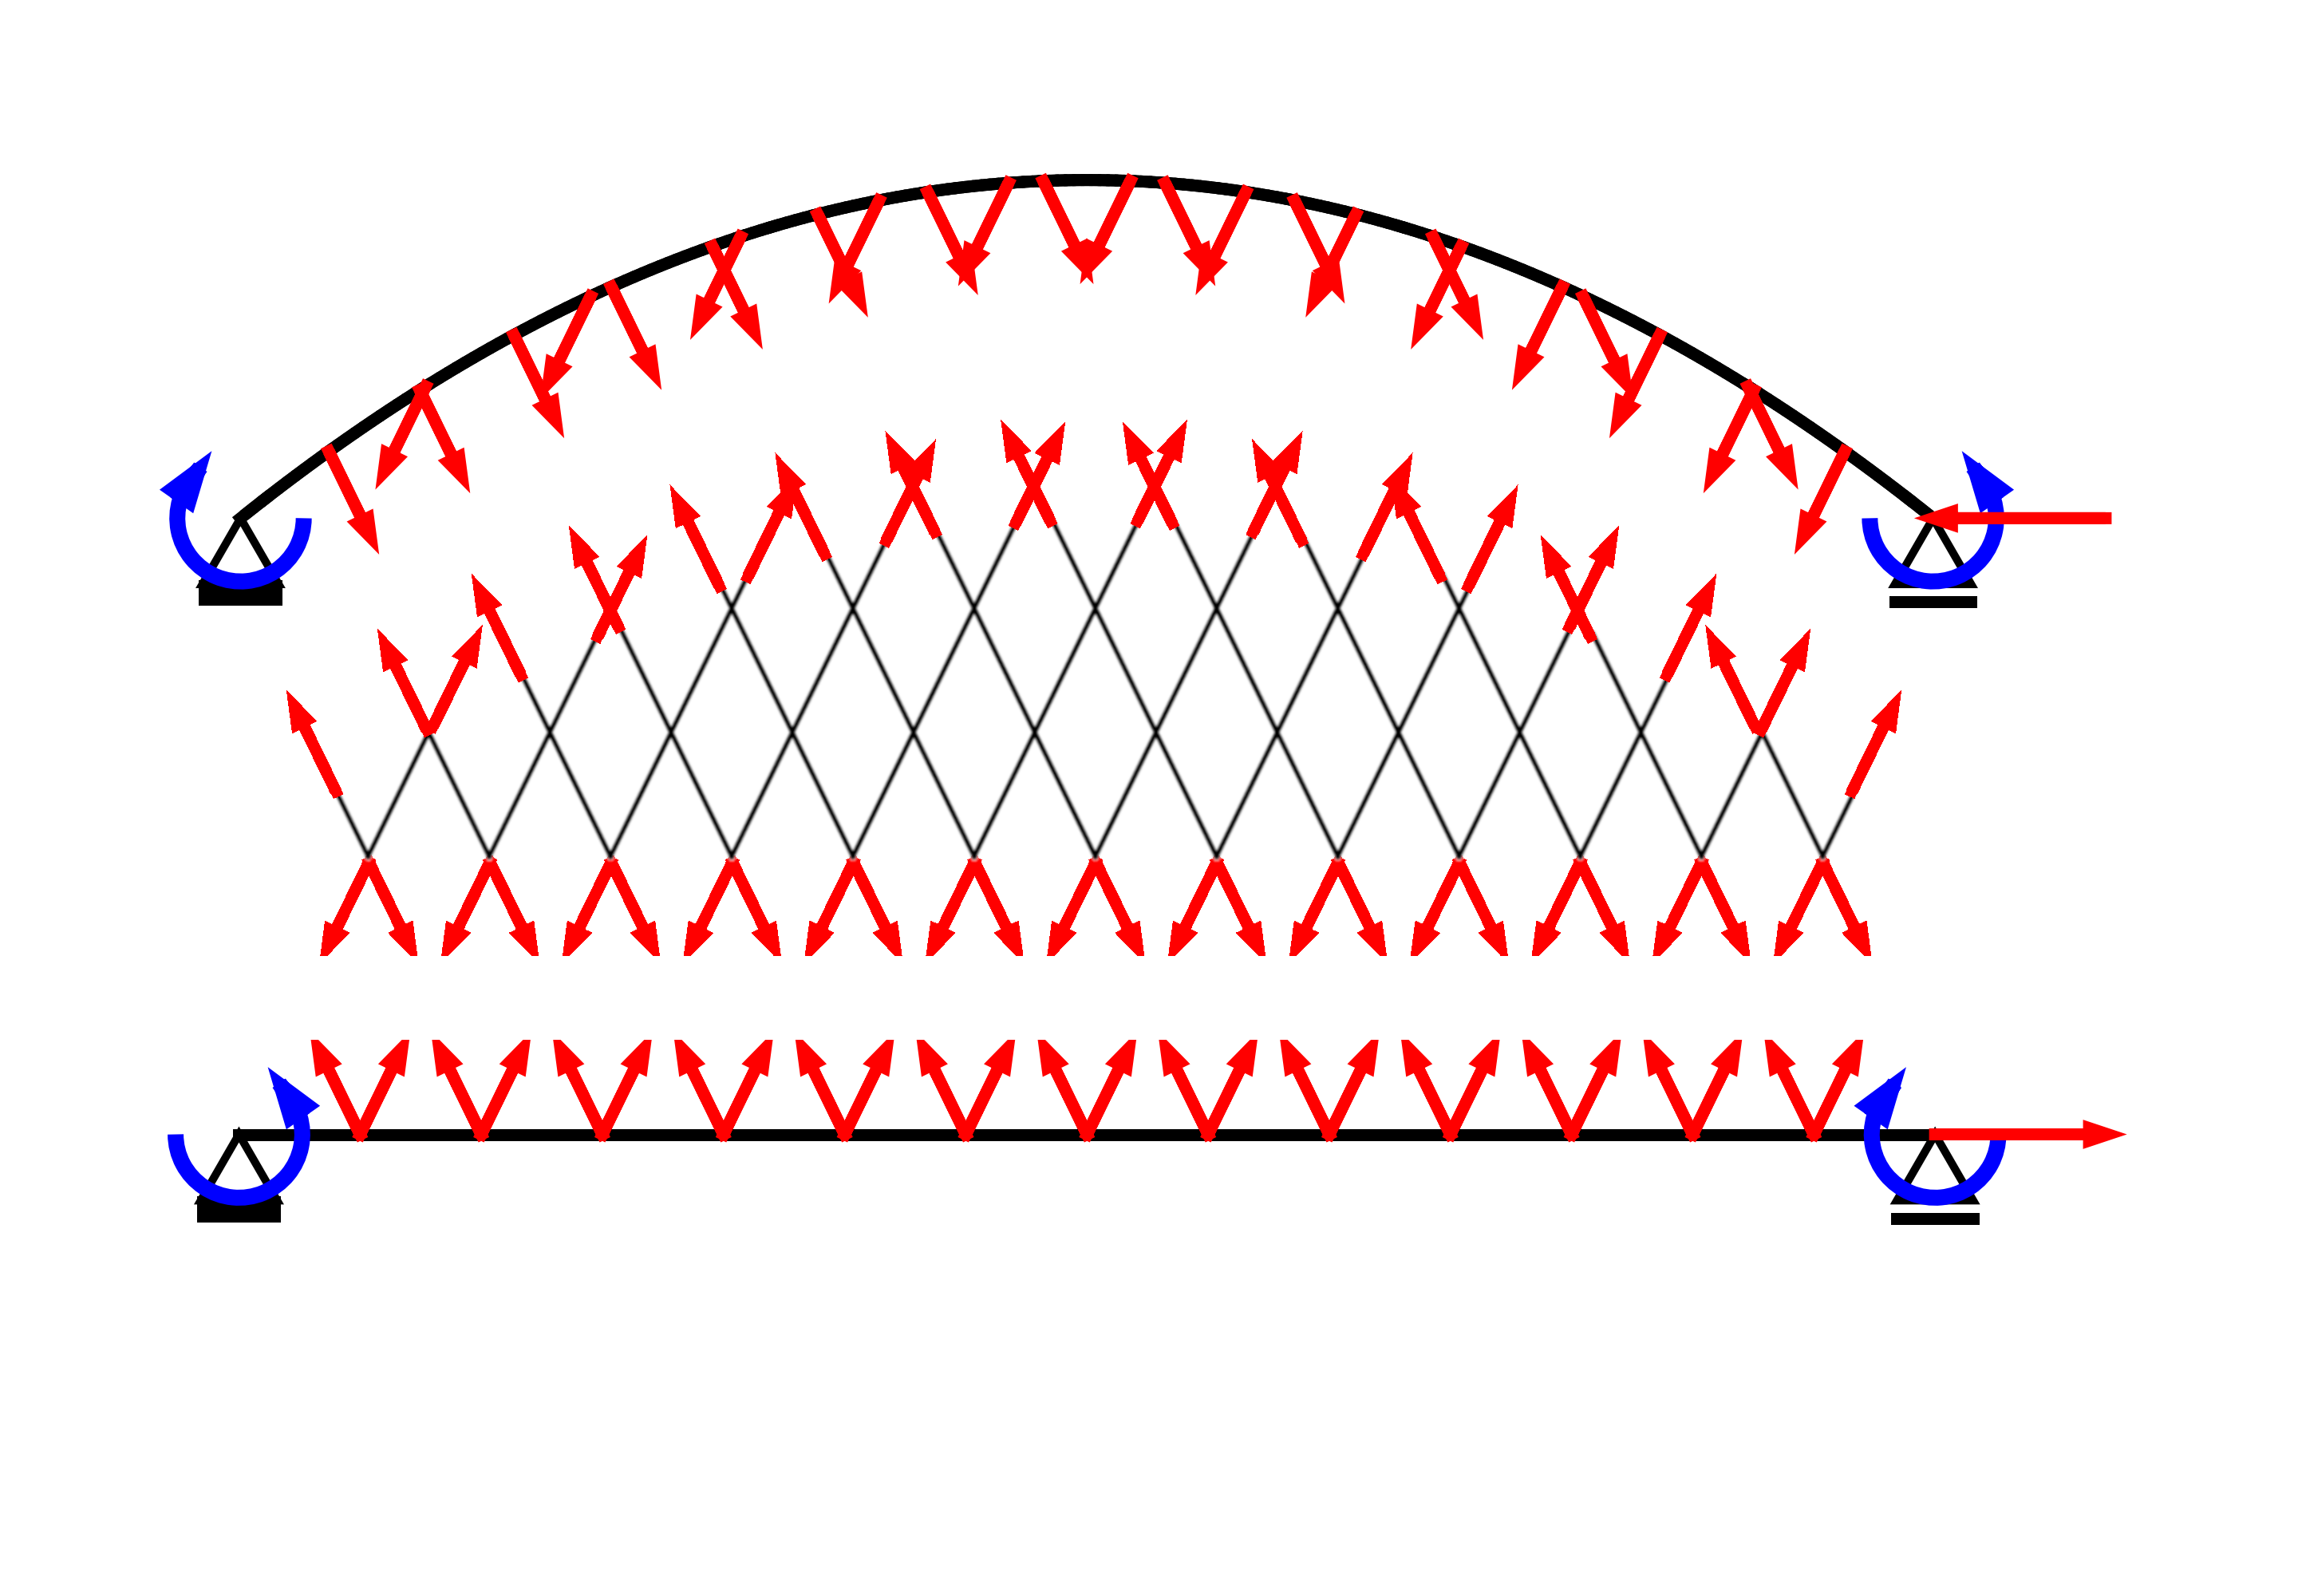
\includegraphics[trim={1cm 16cm 4cm 6.5cm},clip, width=0.57\textwidth]{overleaf/Pictures/Supernumerary forces.png}
    \caption{Set of supernumerary forces in the structural model}
    \label{fig:super_forces}
\end{figure}

For the Blennerhassett Island Bridge, 29 independent self-equilibrium stress states are present, one for each hanger and three between the arch and the tie. Under consideration of symmetry, 15 independent states remain. Instead of the hypothetical residual stress state under no loads, the state under permanent loads defines the self-equilibrium stress state in this Thesis. Thereby, the residual stresses are defined indirectly. 
To investigate the stress state under permanent loads, the model of the network arch bridge is split into the tie and the arch. If the forces at the knuckle and in the hangers are consistent, they can ultimately be recombined to form the permanent state of the network arch.
For general circumstances, including unsuitable arch shapes and hanger arrangements, it is challenging to find appropriate permanent hanger forces. This task is usually tackled by the engineer through trial and error, as it was the case for the design of the Blennerhassett Island Bridge. The respective result is neither reproducible, nor can it claim optimality. Following, a few alternative methods with a variety of applications are presented. 


\subsection{Zero-displacement method}
The zero-displacement method gives a first estimation of the hanger forces and is often used for the more popular cable-stayed bridge type. The permanent hanger forces are determined from a structural analysis of the tie girder in which at every hanger connection a vertical support is introduced. In this way, the moment distribution in the tie is adequately balanced, and creeping effects do not change the moment distribution. For a network tied-arch bridge, additionally to the supports at the connection nodes, a fully fixed support can be introduced at the knuckle. It represents the tie girder's connection to the arch rib and gives the permanent moment between the two, which has also been considered part of the supernumerary set. The model of the tie resembles a multi-span beam, as shown in \cref{fig:zero_disp}. For a network tied-arch bridge, multiple hangers can connect to the tie at a particular node and the vertical forces have to be distributed between the respective hangers. One option is to assign forces of equal magnitude to each of the hangers resulting in the intended vertical force. 

\begin{figure}[H]
    \centering
    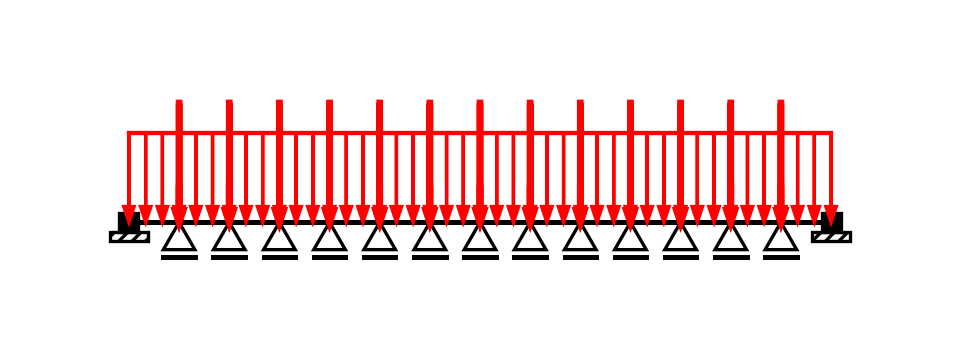
\includegraphics[trim={0 1cm 0 1cm},clip,width=0.6\textwidth]{illustrations/optimisation methods/zero-displacement.png}
    \caption{Zero-displacement method on the tie girder}
    \label{fig:zero_disp}
\end{figure}

In a second step, the hanger forces and the constraint moment at the knuckle are applied to the arch to determine its permanent state. Thereby, the arch is affected by a significant moment distribution with the peak at the crown of $M_{p,crown}$. However, the permanent tie tension force, which has a decisive influence on the arch, can be chosen freely as it was neglected in the tie girder's investigation. As a simplistic approach, the permanent tie tension force $N_{p,Tie}$ can be calculated to cause a disappearing moment at the crown of the arch according to \cref{eq:M_0}. Otherwise, the more elaborate methods of the followings sections can determine the last supernumerary force.

\begin{equation}
    N_{p,Tie} = \frac{M_{p,crown}}{r}
    \label{eq:M_0}
\end{equation}

This fast and simple approach yields adequate permanent moment distributions for a standard hanger arrangement and an adapted arch shape. However, for a radial hanger arrangement, in which the hanger connections do not coincide with the floor beams, or for a specific arch shape that does not resemble the respective thrust line, the zero-displacement method does not give a useful self-equilibrium stress state.

\subsection{Moment minimisation}
It is the goal of an efficient initial configuration to simplify the design verifications by counteracting the effects expected in the various load cases. It can be achieved by minimising the permanent moment distribution in the tie and potentially the arch. Therefor, the permanent moment distribution at m points along the considered component $M \in \mathbb{R}^m$ are described by \cref{eq:perm_mom}. 
\begin{equation}
    {\bf M} = {\bf M_0} + \sum_{i=1}^{n} {\bf M_i} \cdot X_i = {\bf M_0} + {\bf M_{sn}} \cdot {\bf X}
    \label{eq:perm_mom}
\end{equation}
where ${\bf M_0} \in \mathbb{R}^m$ is the moment distribution of the permanent loads on the basic system, ${\bf M_i} \in \mathbb{R}^m$ is the moment distribution of the i-th supernumerary unit force, ${X_i} \in \mathbb{R}$ is the i-th supernumerary force. The latter two can be combined into the matrix of supernumerary moment distributions ${\bf M_{sn}} \in  \mathbb{R}^{m\times n}$ and the vector of supernumerary forces or moments ${\bf X} \in \mathbb{R}^n$. An example of a supernumerary hanger force and its moment distribution is shown in \cref{fig:Minimisation}.

\begin{figure}[H]
\centering
\begin{subfigure}{0.5\textwidth}
    \centering
    \vspace*{0.37cm}
    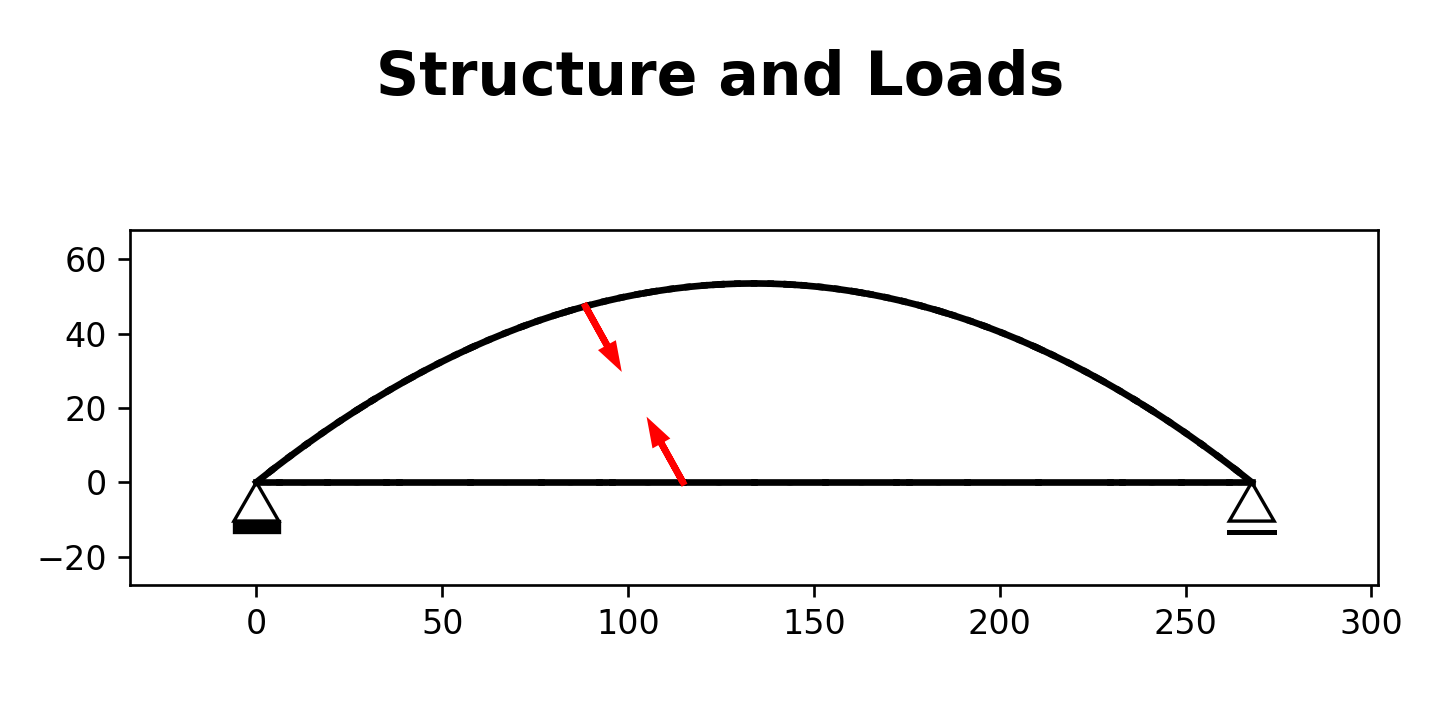
\includegraphics[trim={4cm 3cm 3cm 5.2cm},clip, width=0.88\textwidth]{illustrations/optimisation methods/overall optimisation single force.png}
    \vspace*{0.37cm}
    \caption{Basic system and supernumerary force}
    \label{fig:Minimisation_1}
\end{subfigure}%
\begin{subfigure}{.5\textwidth}
    \centering
    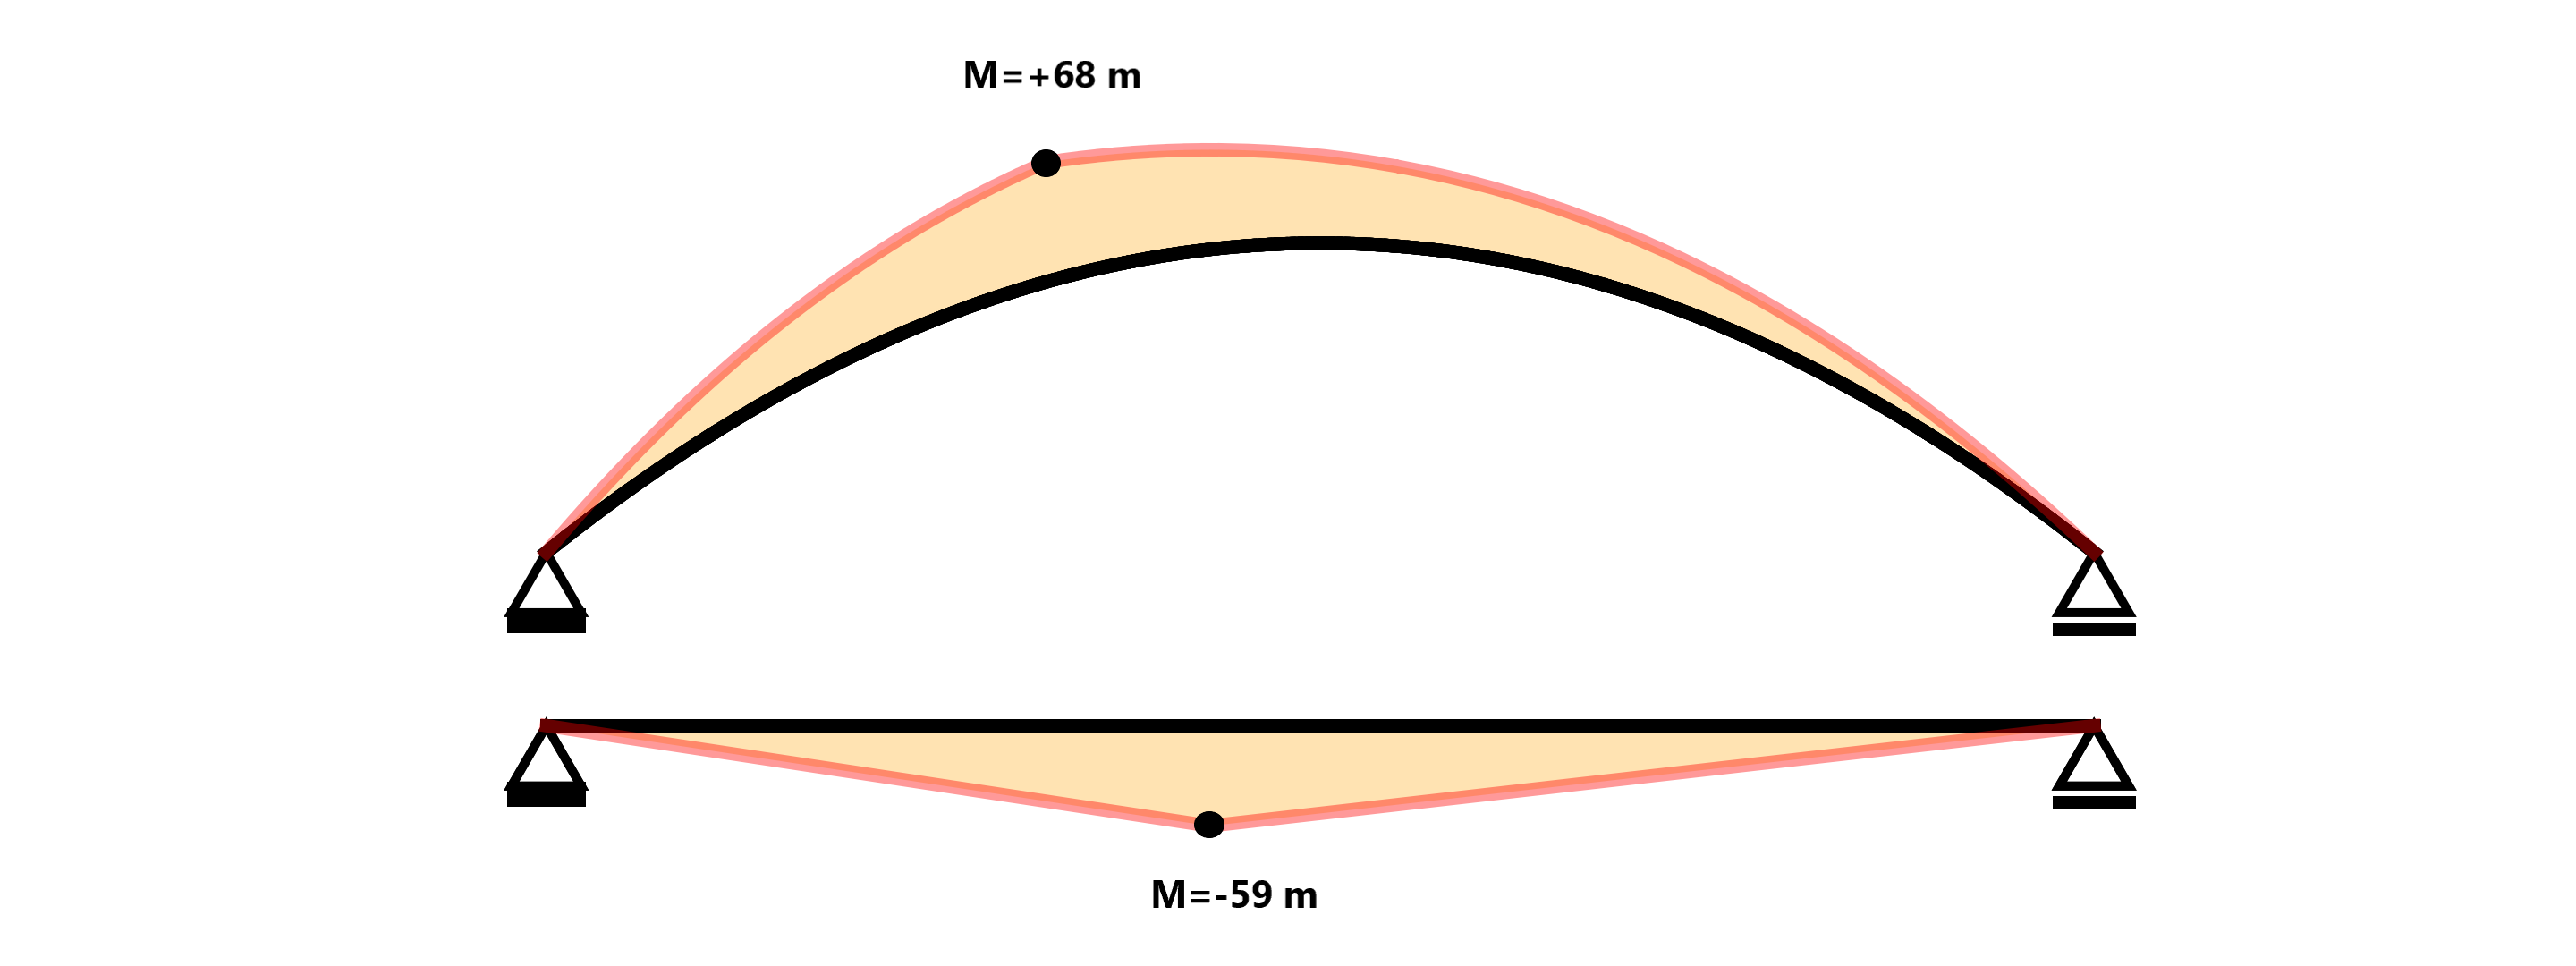
\includegraphics[trim={10cm 1cm 10cm 1cm},clip, width=0.88\textwidth]{illustrations/optimisation methods/overall optimisation single force moment.png}
    \caption{Moments under supernumerary force}
    \label{fig:Minimisation_2}
\end{subfigure}
\caption{Moment distribution of a supernumerary force}
\label{fig:Minimisation}
\end{figure}

The problem of minimising the absolute maximum moments can be formulated according to \cref{eq:minimisation}, where the absolute maximum moment is also expressed as the infinity norm.
\begin{align}
    \underset{{\bf X}}{\text{Minimize}} \quad & f({\bf X}) = \max({\bf M}, -{\bf M}) = \|{\bf M_0} + {\bf M_{sn}} \cdot {\bf X}\|_{\infty} 
    \label{eq:minimisation}
\end{align}
With the helper variable $t$, the previously stated problem can be formulated as a linear programming problem, as shown in \cref{eq:minimisation_2}.
Satisfying the inequality conditions, the variable $t$ describes the moment magnitude which is larger than the all absolute moments in ${\bf M}$.
\begin{align}
    \underset{t, {\bf X}}{\text{Minimize}} \quad & f(t) = t \label{eq:minimisation_2} \\
    \text{s.t.} \quad & {\bf M_0} + {\bf M_{sn}} \cdot {\bf X} - t {\bf 1} \leq  0 \nonumber \\
    \quad & {-\bf M_0} - {\bf M_{sn}} \cdot {\bf X} - t {\bf 1} \leq 0 \nonumber
\end{align}
Additionally, bounds for the permanent hanger forces can be specified as further inequality conditions. It should be noted that under the consideration of symmetry the amount of variables in the linear problem can be reduced. If only the moment distribution in the tie is optimised, it makes sense to only consider vertical forces at each hanger node to obtain an unambiguous problem. In a second step, the optimised vertical forces are assigned to the two hangers at the node. The obtained problem is efficiently and reliably solvable as it is formulated as a linear programming problem. It can even be solved by Microsoft Excel without the need of additional software.

\subsection{Least squares of moments} \label{sec:least_squares}
As an alternative approach, the supernumerary forces can be determined using the method of least squares. This method aims to find supernumerary forces that counteract a particular moment distribution, for example, the moment distribution on the basic system. The objective is described by \cref{eq:lsq_1}, using the variables introduced in the previous section.
\begin{equation}
    {\bf M_{sn}} \cdot {\bf X} = -{\bf M_0}
    \label{eq:lsq_1}
\end{equation}
As this yields an overdetermined system, the equations cannot be solved simultaneously. Using the method of least squares, the sum of the squared deviations can be minimised by solving the determined system in \cref{eq:lsq_2}.
\begin{equation}
    ({\bf M_{sn}}^T\,{\bf M_{sn}}) \cdot {\bf X} = -{\bf M_{sn}}^T\,{\bf M_0}
    \label{eq:lsq_2}
\end{equation}
The drawback of this method is that no bounds for the hanger forces can be specified. However, this method is advantageous if the hanger forces have been optimised by minimising the tie girder's moments. At this point, the tie girder's permanent tension force is still undefined, as it does not affect the moment distribution. It can then be calculated by considering the moment distribution in the arch rib, minimising the squares of its moment distribution. In this case, the approach is fast and can even be solved without linear algebra, as there is only one variable.


\newpage
\section{Arch shape} \label{sec:met_arch}
The optimisation methods introduced in the previous chapter allow finding an efficient self-equilibrium stress state for a given arch shape. It corresponds to finding hanger forces with a resulting thrust line close to the predefined arch shape. However, a more elegant and efficient solution would be an adaptation of the arch shape to the thrust line under permanent loads. 
For a discrete hanger arrangement, the thrust line can be derived according to the method described in \cref{app:discrete}. 
An alternative method is the derivation of the thrust line for the hypothetical case of an infinitely dense hanger arrangement, which is shown in \cref{sec:continuous}.
Both methods take the weight of the arch into account which compels an iterative derivation.
Ultimately, a polynomial approximation of discrete arrangements is introduced in \cref{sec:polynomial_approximation}

\subsection{Thrust line of discrete hanger arrangement} \label{app:discrete}

Calculating the thrust line of a discrete hanger arrangement is a particular challenge as it is not known in which order the hangers intersect the thrust line beforehand. Therefore it is calculated in steps. It is started from the crown with an estimated normal force $N_{crown}$. The inclination at the beginning of every step corresponds to the ratio of the normal force components $N_x$ and $N_y$. Further, the arch's weight per horizontal meter is estimated from \cref{eq:g_arch}.

\begin{equation}
    g_{arch,x} = g_{arch} \cdot \sqrt{1+y'^2} = g_{arch} \cdot \sqrt{1+\left( \frac{N_{y}}{N_{x}} \right)^2}
    \label{eq:g_arch}
\end{equation}

The parabolic thrust line can be estimated according to \cref{eq:discrete} using the weight per horizontal meter. The height at the beginning of the current step is given by $y_1$. The second term gives the normal force's inclination, which would continue the thrust line under no additional loading. The weight of the arch causes a slight curvature according to the third quadratic term.

\begin{equation}
    y(x) = y_1 - \frac{N_y}{N_x} \cdot x - \frac{g_{arch,x}}{2\cdot N_x}\cdot x^2
    \label{eq:discrete}
\end{equation}

Unless a hanger intersects the thrust line within the current step, the thrust line is continued by the step length $dx$. Considering a linearly discretised arch, the points derived from \cref{eq:discrete} give the exact thrust line. A slight deviation occurs through the inaccurately assumed arch weight if a continuously curved arch is fitted through the obtained points. This deviation can be controlled by a sufficiently small step length $dx$. The obtained point serves as a starting point for the next step for which the vertical component of the normal force is adapted by the arch's weight of the performed step. An illustration is given in \cref{fig:discrete_1}.

\begin{figure}[H]
    \centering
    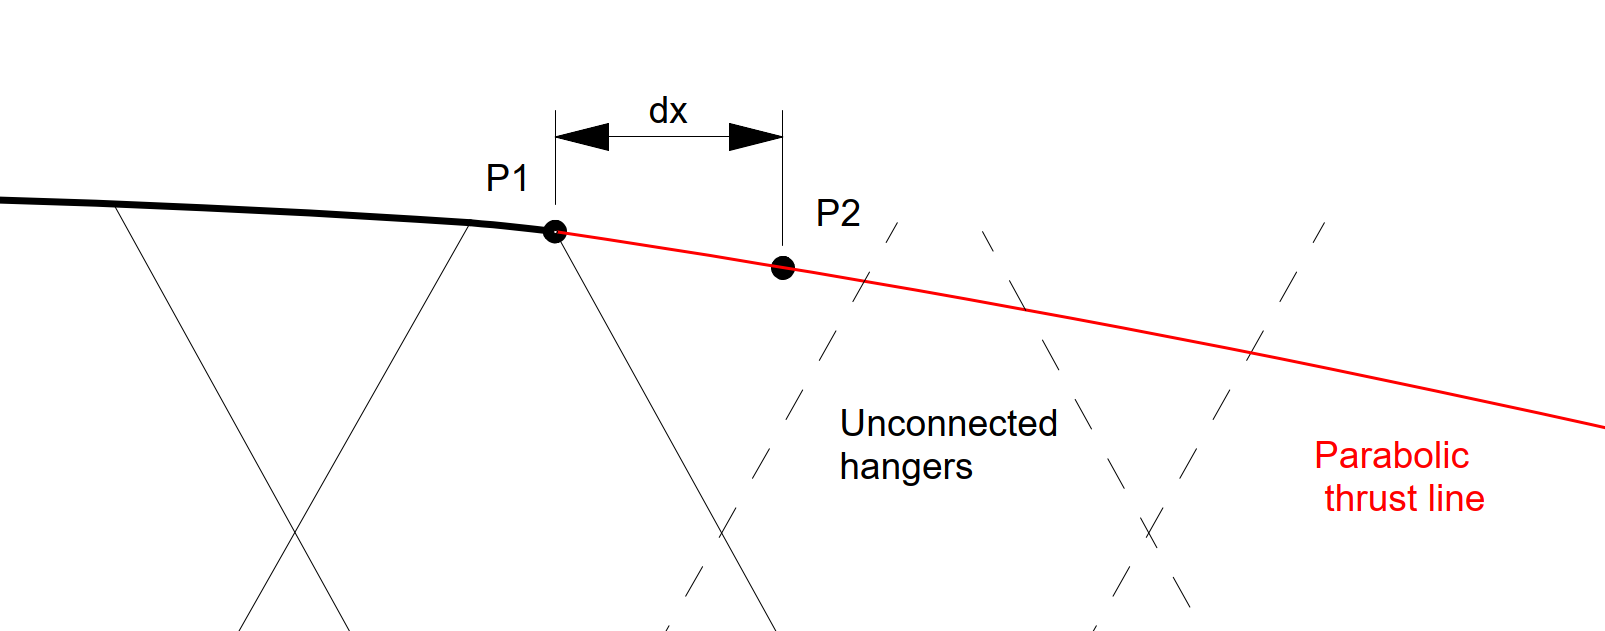
\includegraphics[width=0.7\textwidth]{overleaf/Appendix/Pictures/discrete_thrust_line_1.PNG}
    \caption{Thrust line derivation step without intersecting hangers}
    \label{fig:discrete_1}
\end{figure}

However, if a hanger intersects the thrust line within the current step, this intersection point is added to the thrust line and used as a starting point for the next step. Therefore, the normal force is adapted by the weight of the arch and the hanger force. This step is illustrated in \cref{fig:discrete_2}.

\begin{figure}[H]
    \centering
    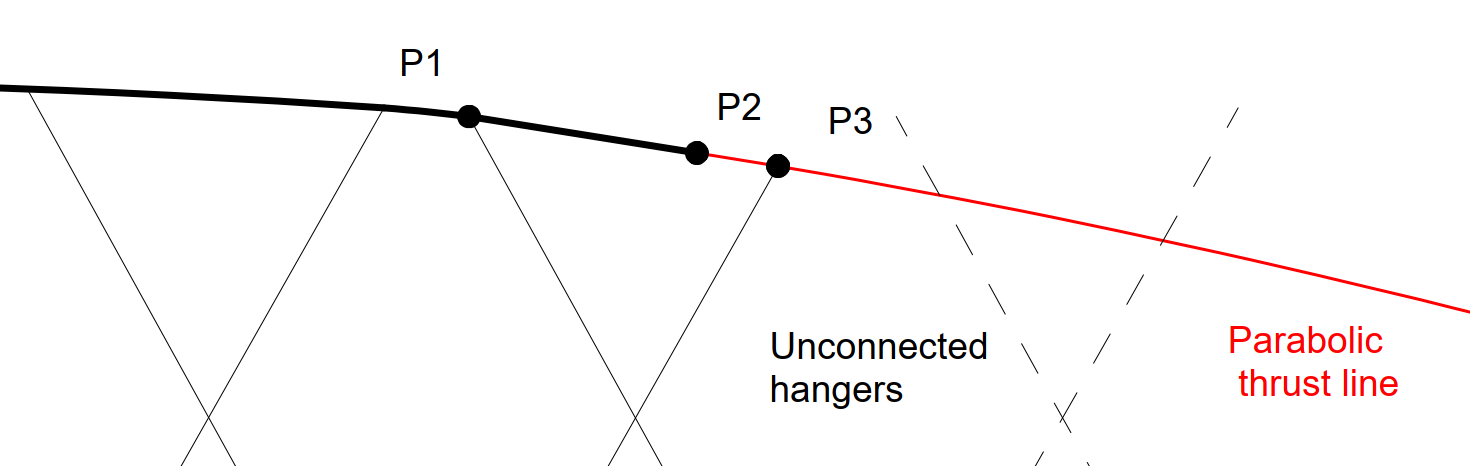
\includegraphics[width=0.65\textwidth]{overleaf/Appendix/Pictures/discrete_thrust_line_2.PNG}
    \caption{Thrust line derivation step connecting to the next hanger}
    \label{fig:discrete_2}
\end{figure}

The normal force in the crown $N_{crown}$ is determined iteratively as the arch weight's distribution is not known beforehand. In each iteration, the crown's normal force can be estimated by the expression in \cref{eq:accurate_n_crown} where $H^*$ is the set of hangers intersecting the axis of symmetry. $F_h$, $\alpha_h$ and $y_h$ give the force, the inclination and the height at midspan of hanger $h$. $M_{mid,glob}$ describes the global moment at midspan and can be derived from \cref{eq:accurate_m_crown}.

\begin{equation}
    N_{crown} = \frac{{M_{mid,glob}+\sum\limits_{h\in H^*}^{}F_h\,\cos(\alpha_h)\,y_h}}{r}
    \label{eq:accurate_n_crown}
\end{equation}
\begin{equation}
    M_{mid,glob} = \frac{(g_{tie}+g_{deck}+g_{util})\,s^2}{8} + M_{mid,arch}
    \label{eq:accurate_m_crown}
\end{equation}

In the first iteration, the expression in \cref{eq:moment_arch_simplified} can be used to estimate the global moment due to the weight of the arch $M_{mid,arch}$. It is derived from the simplified weight distribution of a parabolic arch.
\begin{equation}
    M_{mid,arch}=-g_{arch}\cdot\frac{s\cdot(2r+3s)}{24}
    \label{eq:moment_arch_simplified}
\end{equation}

For the next iterations, the global moment due to the distributed arch weight is determined from the integration given in \cref{eq:moment_arch_exact}.
\begin{equation}
    M_{mid,arch}= 2\,g_{arch}\,\int_{0}^{s/2} \frac{x}{2}\,\sqrt{1+y'(x)^2} \,dx
    \label{eq:moment_arch_exact}
\end{equation}

Alternatively, the correct $N_{crown}$ can be determined numerically as the value for which the thrust line intersects the knuckle point. Therefore, it is advantageous if the knuckle's constraint moment is transformed into a statically equal permanent force in the web plates. While it does not represent a realistic flow of forces, it facilitates the derivation of an adequate arch shape.


\subsection{Thrust line of continuous hanger arrangement} \label{sec:continuous}
For the continuous arrangement, the hanger forces are replaced by hanger force densities $f_l$ and $f_r$ of the two hanger sets, which are determined in a first step. This is done without the consideration of the arch, and there are multiple possibilities to do so. For example, they could be calculated to be in equilibrium with the permanent vertical force $q$. However, horizontal equilibrium is an unnecessary condition, as the tie girder is affected by significant tension forces in any case. Therefore, it is proposed to assign force densities of identical magnitude to the hangers on each infinitesimal element. An illustration with the resultant forces $F_L$ and $F_R$ and the inclination of the hanger sets $\alpha$ and $\beta$ is shown in \cref{fig:continuous_1}.
\begin{figure}[H]
    \centering
    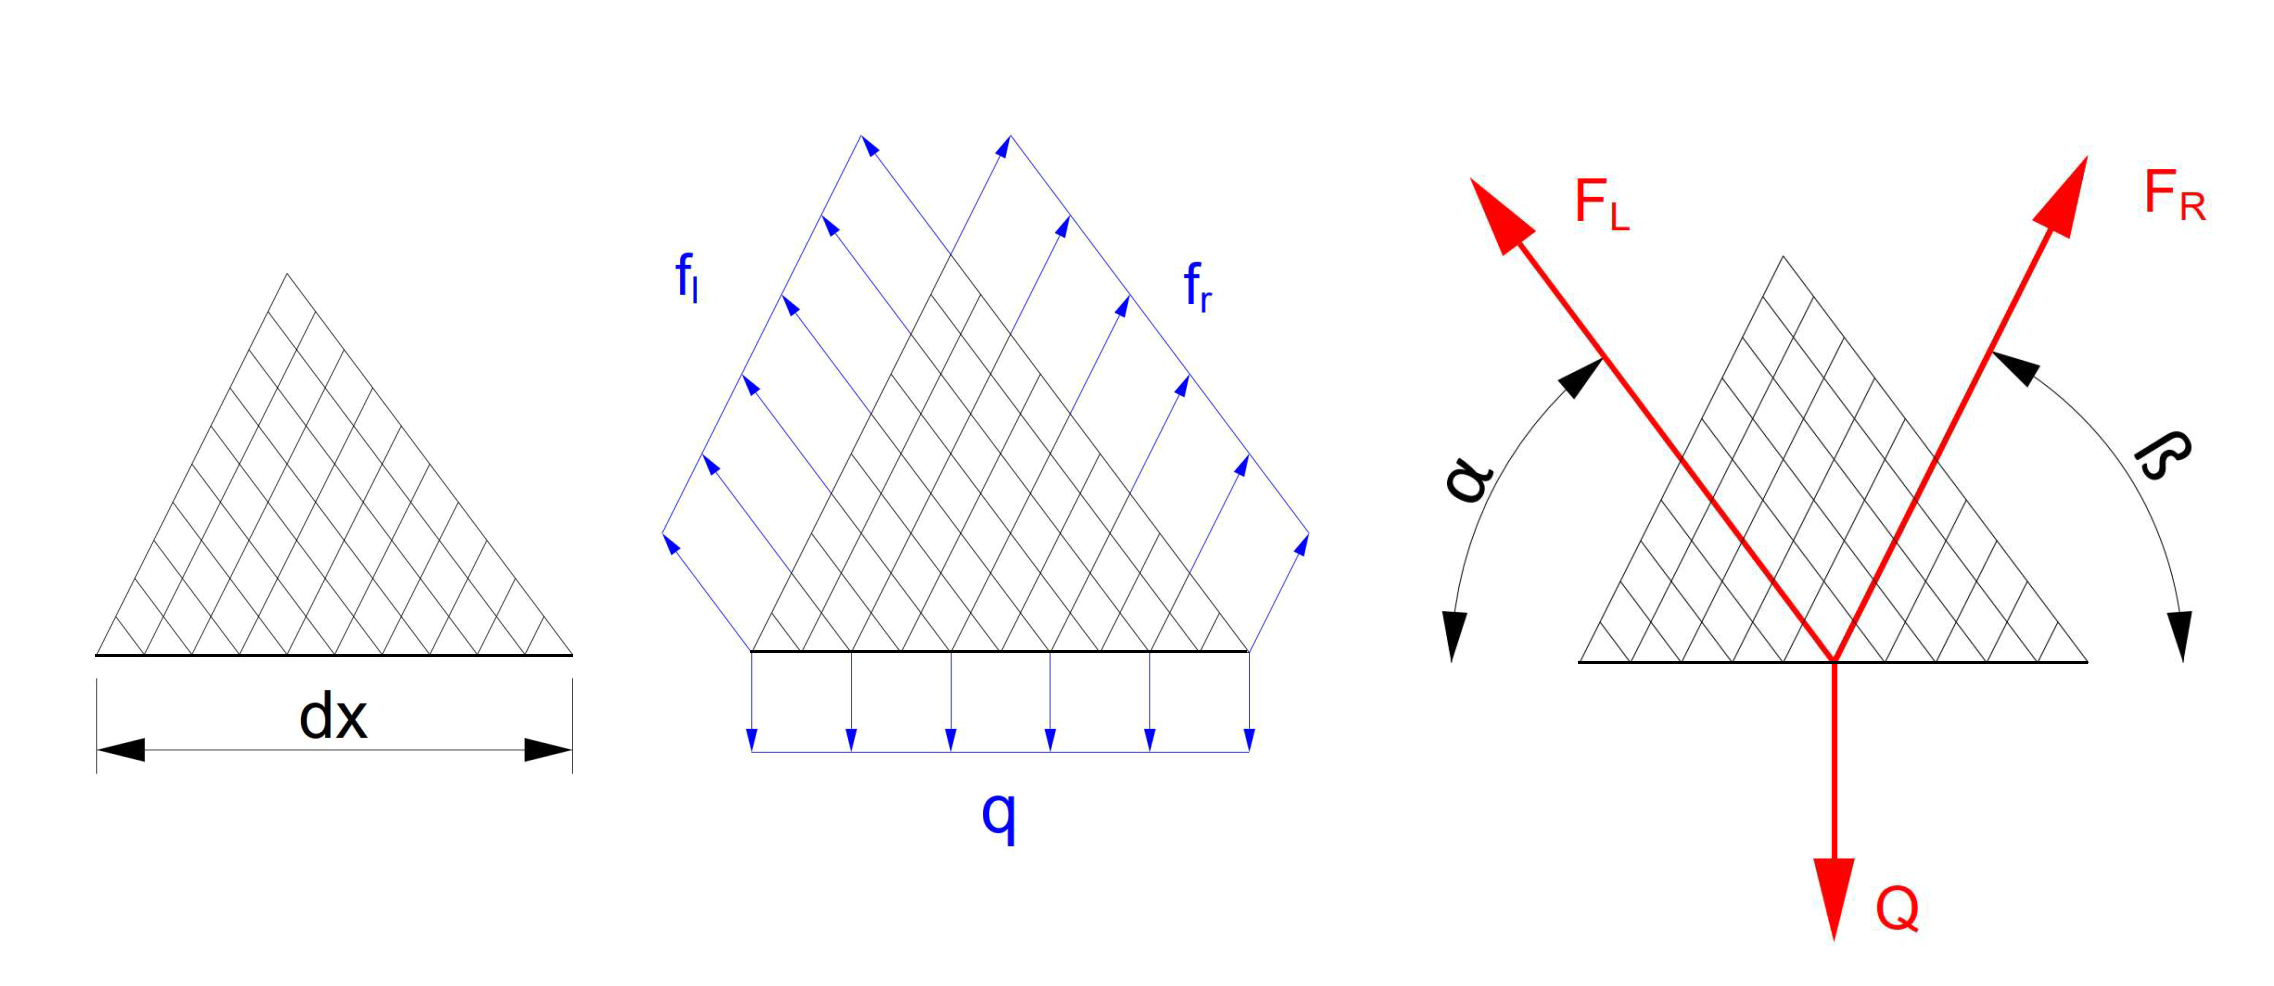
\includegraphics[trim={0 0.5cm 0 1.8cm},clip, width=0.6\textwidth]{overleaf/Appendix/Pictures/continuous_thrust_line_1.PNG}
    \caption{Hanger force densities on an infinitesimal element}
    \label{fig:continuous_1}
\end{figure}

The force densities of equal magnitudes resulting in vertical equilibrium are calculated by \cref{eq:continuous_1}.
\begin{equation}
    f_l=f_r=\frac{q}{\sin{\alpha}+ \sin{\beta}}
    \label{eq:continuous_1}
\end{equation}

A differential equation can be derived to describe the arch's thrust line. However, it is impossible to get an analytical solution for general hanger arrangement patterns. Therefore, the continuous hanger arrangement's thrust line is also calculated in fixed horizontal steps of $dx$ starting from the crown, where a horizontal normal force $N_{crown}$ is assumed. At the beginning of each step, the normal force $N_1$ is known, and its inclination corresponds to the thrust line's inclination. 
If the step $dx$ is small, it can be assumed that the thrust line's inclination undergoes small changes in every step. In this case, the arch's weight and the applicable hanger forces can be determined from the initial inclination. 
The lengths on the tie girder that affect the considered arch segment $dl_1$ and $dl_2$ are determined from geometrical considerations in order to calculate the hanger forces. With the initially defined hanger force densities, the resultant hanger forces are determined as well as the new normal force $N_2$. A single step is illustrated in \cref{fig:continuous_2}.

\begin{figure}[H]
    \centering
    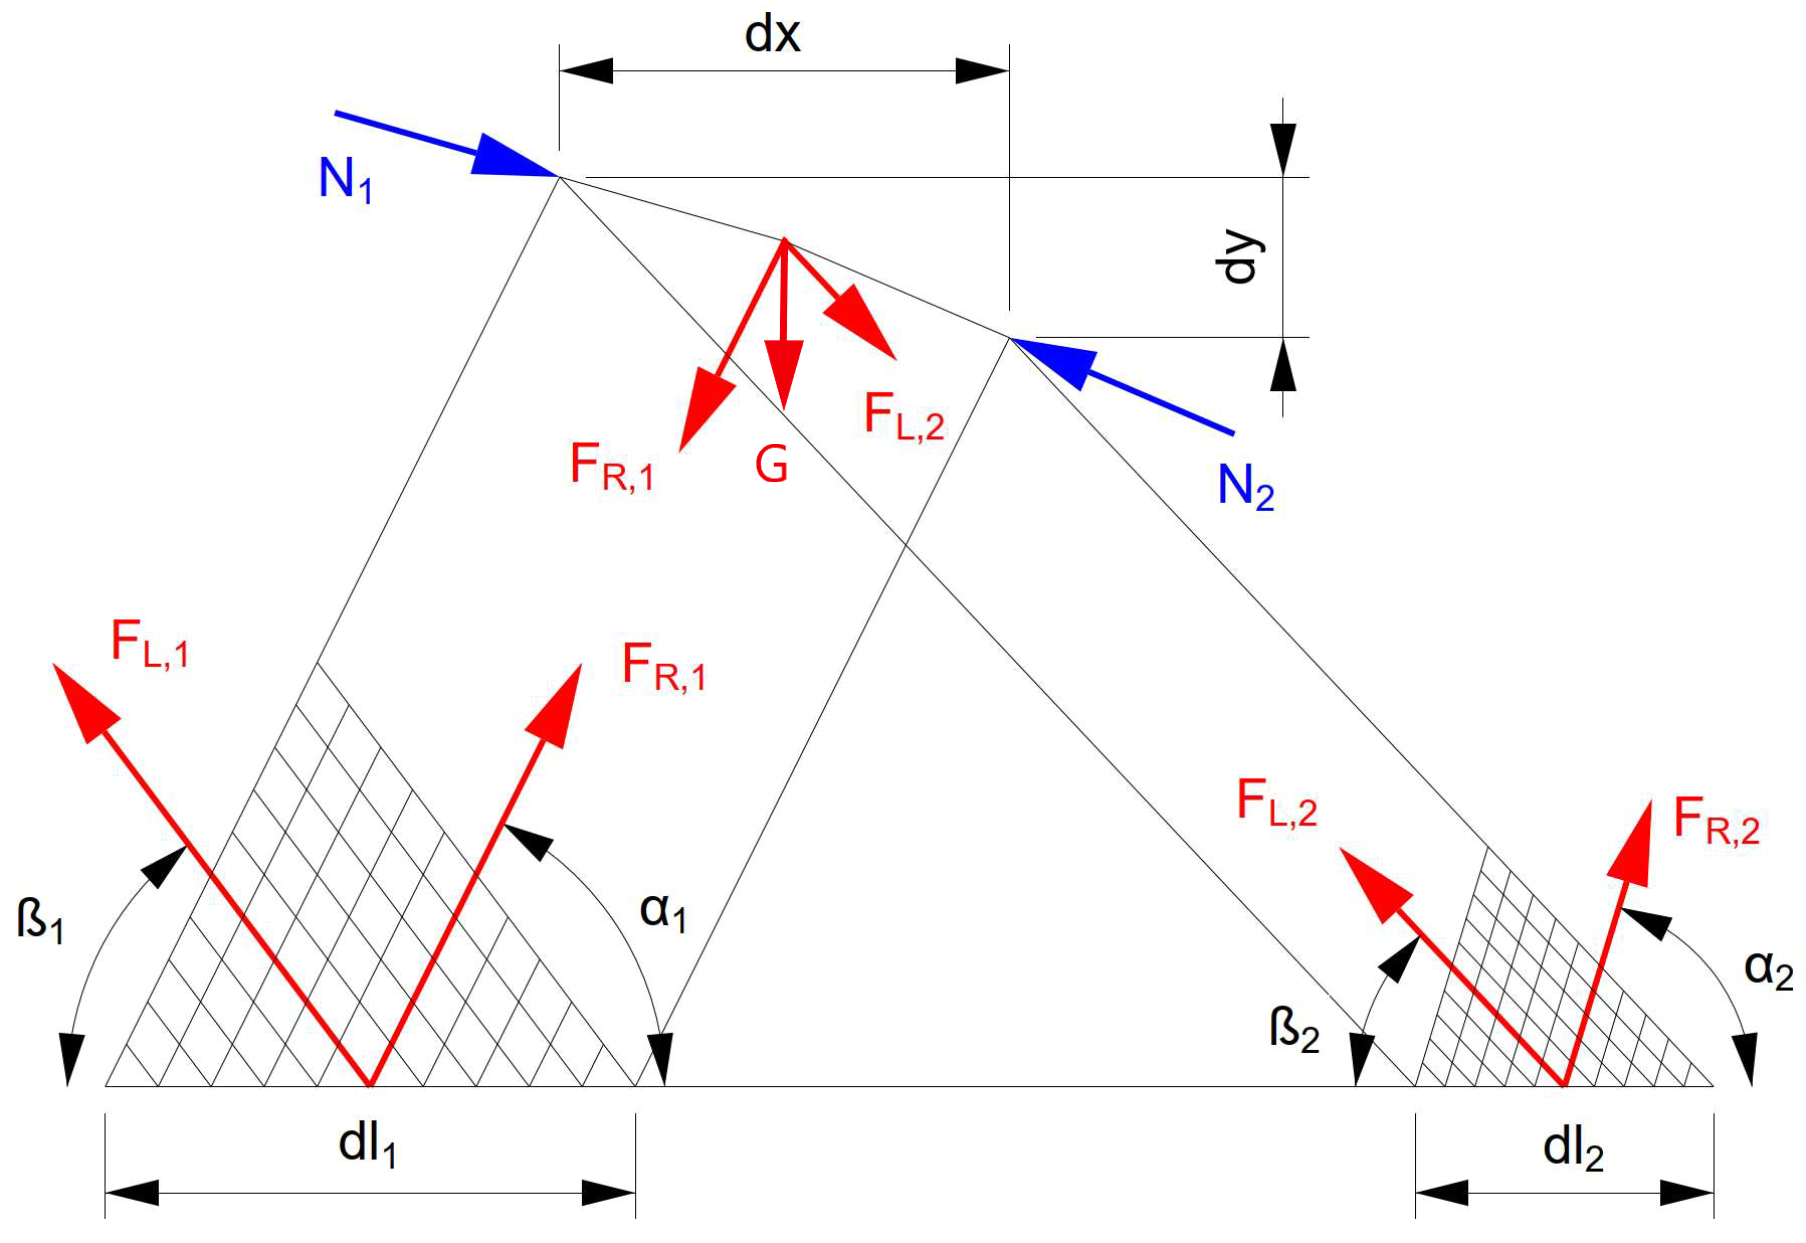
\includegraphics[width=0.58\textwidth]{overleaf/Appendix/Pictures/continuous_thrust_line.PNG}
    \caption{Derivation of the arch thrust line for a continuous hanger arrangement}
    \label{fig:continuous_2}
\end{figure}

Each step solves for the change of height of the thrust line $dy$. It underlies the condition that the new inclination coincides with the inclination of the new normal force $N_2$, which is described by \cref{eq:continuous_2}.
\begin{equation}
    dy = \frac{dx}{2} \cdot \left(\frac{N_{1,y}}{N_{1,x}} + \frac{N_{2,y}}{N_{2,x}} \right)
    \label{eq:continuous_2}
\end{equation}


Unless the arch's weight is neglected, the normal force in the crown $N_{crown}$ is determined iteratively for the thrust line to intersect the knuckle point. Another possibility is its determination from static considerations similar to the ones in the previous section.

\subsection{Polynomial approximation} \label{sec:polynomial_approximation}
While the previously derived discrete hanger arrangement thrust line is certainly efficient it lacks constructability. The kinks resulting from the hanger forces do not comply with the cutting and welding methods used for building the cross section. Further, a kinked arch would look particularly unaesthetic. Therefore, the arch shape specified by the discrete arch nodes is approximated by a function with a continuous curvature. The parabola and the circular arc lack a parameter to fit the curve to the obtained nodes. As the cubic polynomial is not symmetric and therefore unsuitable, the quartic polynomial is the apparent choice. It is expressed by \cref{eq:polynomial_shape} with the origin at midspan in the tie girder.
\begin{equation}
    y(x)=r \cdot \left(1 - b \cdot \left(\frac{2\,x}{s}\right)^2 - (1-b) \left(\frac{2\,x}{s}\right)^4 \right)
    \label{eq:polynomial_shape}
\end{equation}

It fulfills the conditions $y(0)=r$ and $y(s/2)=y(-s/2)=0$. The shape parameter $b$ determines the shape between these points. A value of $b=1$ yields a parabola whereas a value of $b=0$ yields a purely quartic shape function. A comparison of the shapes for the case of the Blennerhassett Island Bridge is given in 

\begin{figure}[H]
    \centering
    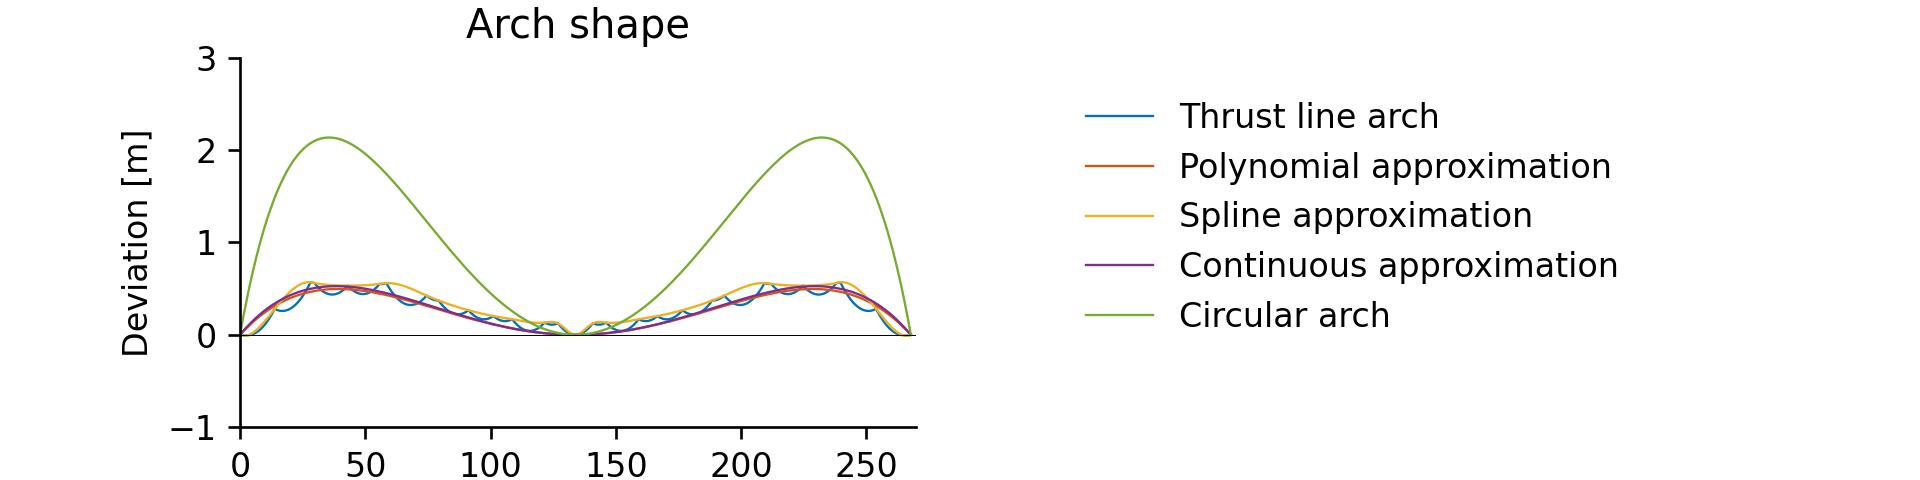
\includegraphics[trim={1cm 0 3cm 0},clip, width=0.76\textwidth]{calculations/arch shape/arch_shapes_13.png}
    \caption{Deviation of the polynomial approximations to the parabola}
    \label{fig:arch_shapes_13}
\end{figure}

\newpage
\section{Design verifications} \label{sec:met_ver}
To ensure a safe and reliable structure, the limit states for strength, extreme events and fatigue are considered \cite{AASHTO}.  The resulting demand over capacity ratios (D/C) will also be used in \cref{sec:met_cost} for an estimation of the cost function.

\subsection{Strength limit states}
The strength limit states are considered to ensure that the design of the structure guarantees enough strength and stability for the highest expected loads in its life cycle. The load combinations considered in this investigation are related to the main actions of vehicular use (Strength-I), wind exposure (Strength-III) and a load combination for heavy bridges (Strength-IV). The load factors used for each strength limit state are presented in \cref{tab:uls_combination}. For the permanent loads DC and DW, two factors are given out of which the one impeding to the verification is taken. For the locked-in erection stresses no variability is taken into account.

\begin{table}[H]
\caption{Load combinations for the ultimate limit state}
\centering
\begin{tabular}{lccccc}
\hline
Load         & EL  & DC         & DW         & LL   & WS  \\ \hline
Strength-I   & 1.0 & 0.9 / 1.25 & 0.65 / 1.5 & 1.75 & -   \\
Strength-III & 1.0 & 0.9 / 1.25 & 0.65 / 1.5 & -    & 1.4 \\ 
Strength-IV  & 1.0 & 0.65 / 1.5 & 0.65 / 1.5 & -    & - \\ \hline
\end{tabular}
\end{table}

The arch and the tie are verified according to \cref{eq:design_verification}, neglecting the secondary force effects. For the hangers, enough resistance is proved if the highest stresses are below 65\% of the nominal capacity. 

\begin{equation}
    \frac{N_{Ed}}{N_{Rd}} + \frac{8.0}{9.0}\, \left(\frac{M_{y,Ed}}{M_{y,Rd}}+\frac{M_{z,Ed}}{M_{z,Rd}} \right) \leq 1.0
    \label{eq:design_verification}
\end{equation}

For simplicity, the value given by the left side of this condition is also referred to as the demand over capacity ratio for the arch and the tie.
%For the Blennerhassett Island Bridge, the DOC is evaluated according to this simplified verification. The obtained values are presented in Table [], along with the ratios taken from the design drawings in parenthesis. 

\subsection{Extreme event limit states}
Extreme events are unique circumstances whose return periods can be significantly greater than the life expectancy of the structure. In these events, the requirement for the bridge is its structural survival. In this investigation the extreme events of cable loss, cable replacement and tie fracture are examined. The load factors for each event is taken from the design drawings and presented in \cref{tab:extreme_combination}. For the events of cable loss and cable replacement, specific live loading arrangements (LL*) apply.

\begin{table}[H]
\caption{Load combinations for the extreme event limit states}
\label{tab:extreme_combination}
\centering
\begin{tabular}{lccccc}
\hline
Event         & EL  & DC         & DW         & LL*   & DAF  \\ \hline
Cable loss   & 1.0 & 1.2 & 1.4 & 0.75 & 1.75   \\
Cable replacement & 1.0 & 1.2 & 1.4 & 1.5 & 1.0 \\ 
Tie fracture  & 1.0 & 1.25 & 1.5 & 1.3 & - \\ \hline
\end{tabular}
\end{table}

For both hanger-related extreme events, each hanger is investigated individually according to the PTI (static) approach [cite PTI]. In a first step, the longitudinal live load arrangement, which maximises the respective hanger force, is determined. Therefor, The concentrated live load is always applied at the cross-girder closest to the considered hanger. The forces from the distributed live load are also arranged on a certain amount of neighbouring cross-girders, as illustrated in \cref{fig:Cable_Loss_1}. The assumed hanger force before its replacement or loss is thereby determined. In a second step, the structural system is modified by removing the considered hanger. The hanger force is applied in opposite direction on the modified system, as shown in \cref{fig:Cable_Loss_2}. The resulting effects are multiplied by a dynamic amplification factor (DAF) and superimposed on the effects from the state of maximised hanger force. The DAF for the event of cable loss is assumed to be 1.75.

\begin{figure}[H]
\centering
\begin{subfigure}{0.5\textwidth}
    \centering
    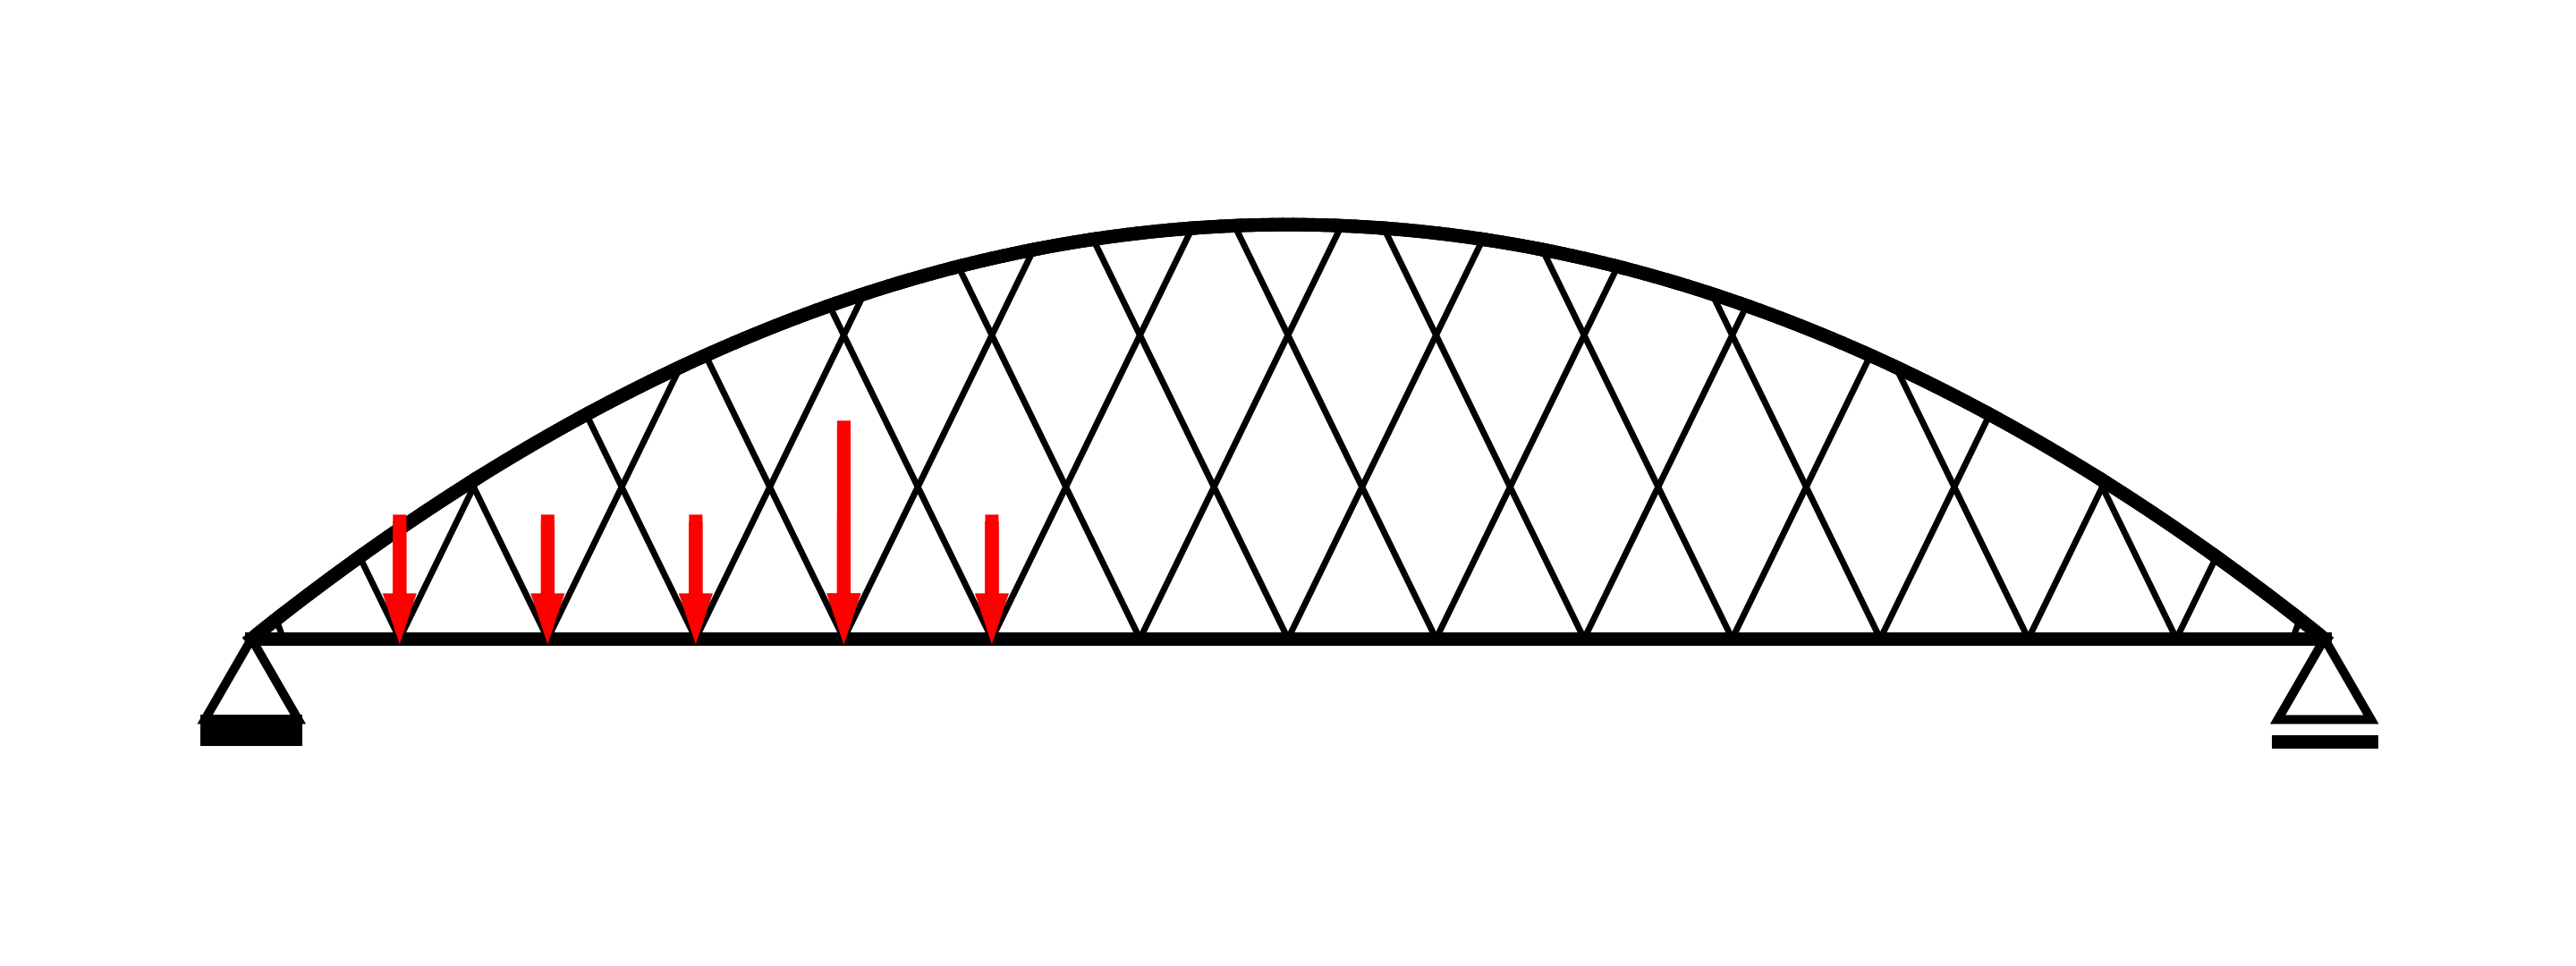
\includegraphics[trim={0 0.8cm 0 0.8cm},clip, width=0.9\textwidth]{illustrations/figures/cable loss - load arrangement.png}
    \caption{Live load arrangement to maximise hanger force}
    \label{fig:Cable_Loss_1}
\end{subfigure}%
\begin{subfigure}{.5\textwidth}
    \centering
    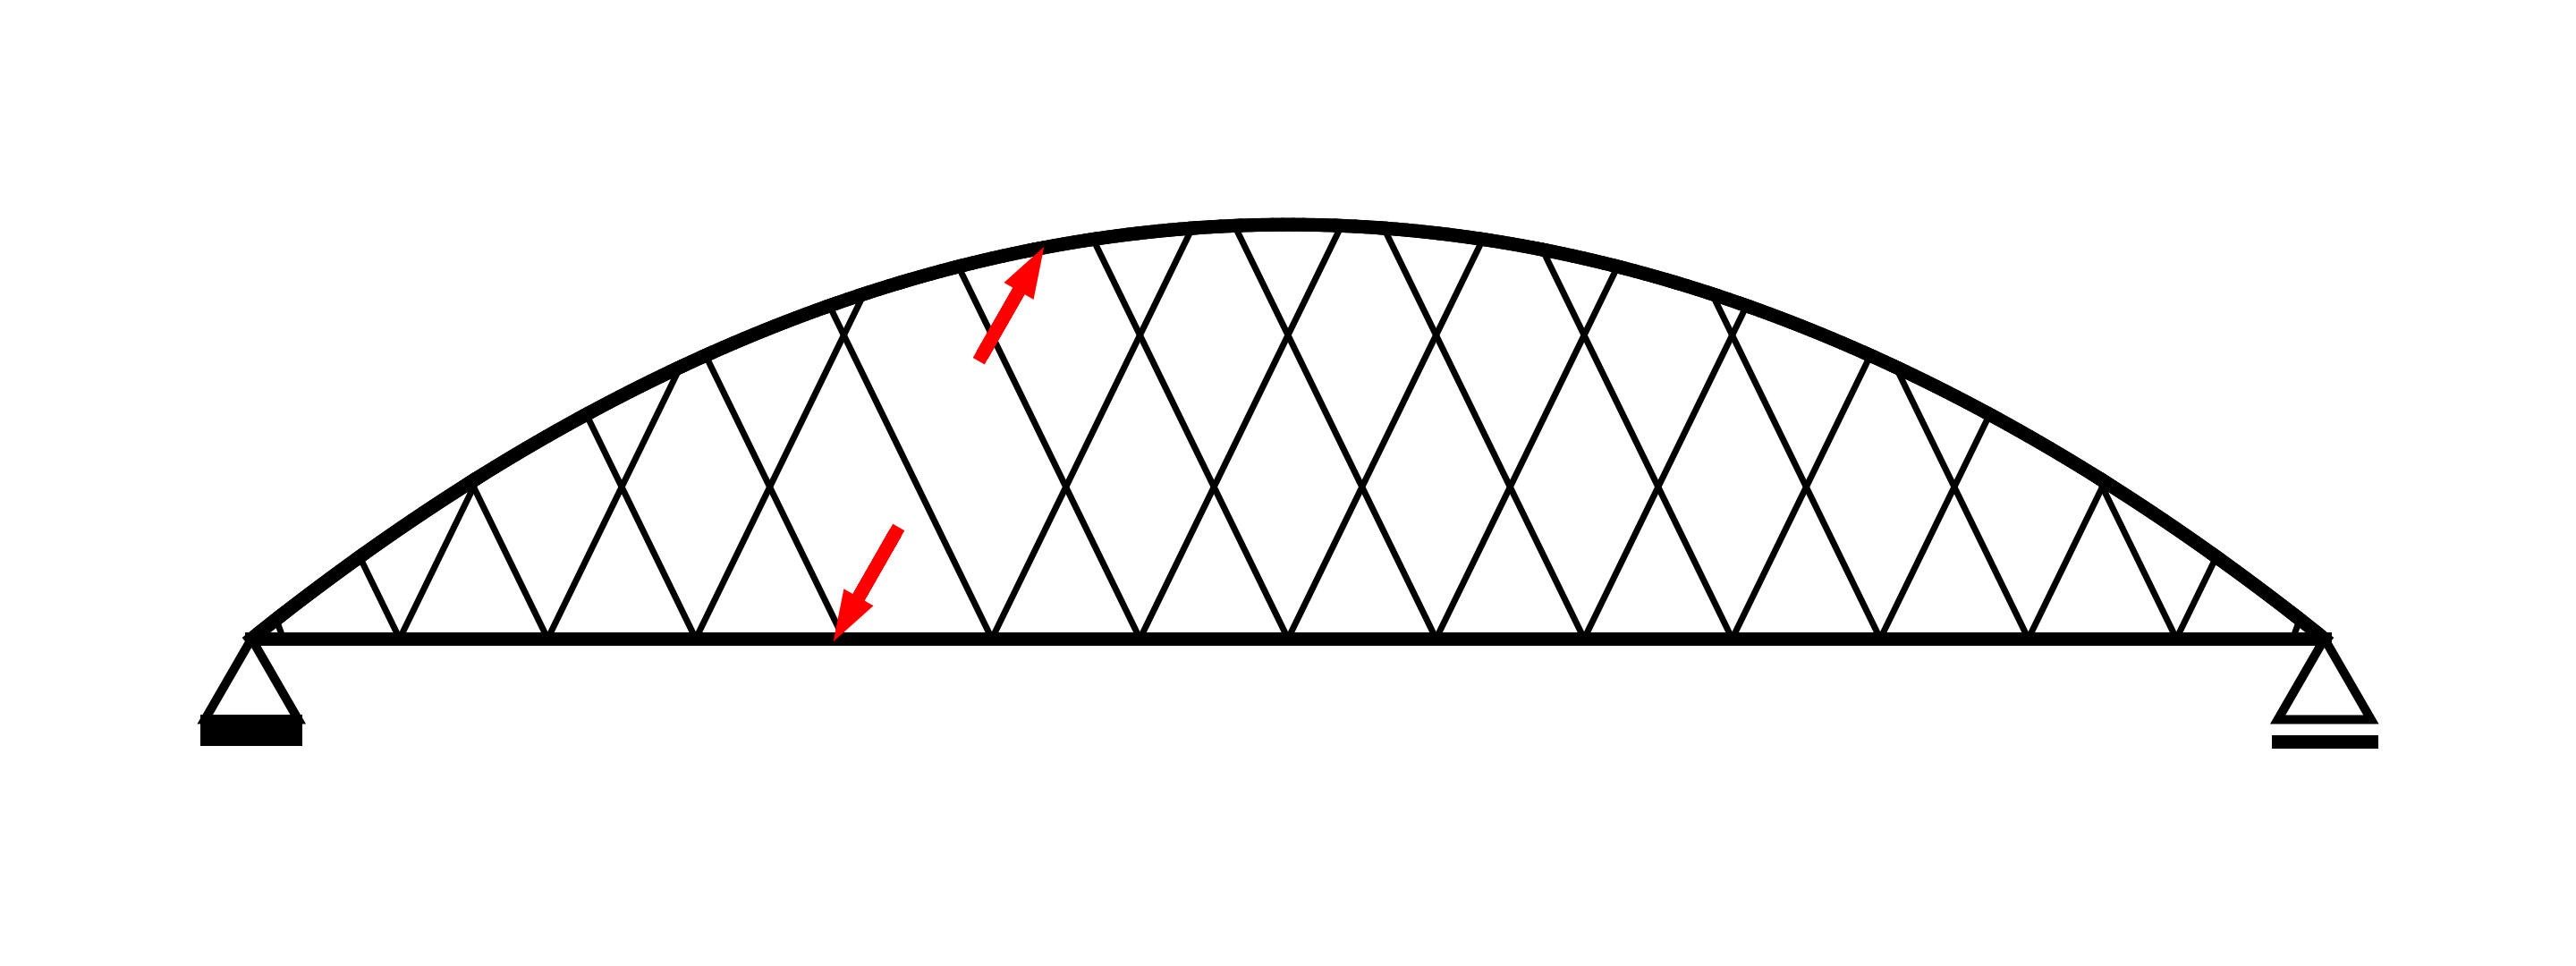
\includegraphics[trim={0 0.8cm 0 0.8cm},clip, width=0.9\textwidth]{illustrations/figures/cable loss.png}
    \caption{Structural model with opposite force}
    \label{fig:Cable_Loss_2}
\end{subfigure}
\caption{Calculation steps for loss of the fourth hanger}
\label{fig:Cable_Loss}
\end{figure}

[Tie fracture]

\subsection{Fatigue limit state}

\begin{table}[H] 
\caption{Cross-sectional resistances}
\centering
\begin{tabular}{lccc}
\hline
Segment & Normal force & Moment-y & Moment-z \\
 & [MN]   & [MNm] & [MNm] \\ \hline
Arch 1 & \SI{130.0}{} & \SI{78.7}{} & \SI{79.1}{}\\
Arch 2 & \SI{108.8}{} & \SI{71.5}{} & \SI{63.4}{}\\
Arch 3-4 & \SI{82.3}{} & \SI{50.0}{} & \SI{42.7}{}\\
Tie 1 & \SI{153.2}{} & \SI{100.8}{} & \SI{76.2}{}\\
Tie 2 & \SI{117.1}{} & \SI{82.8}{} & \SI{56.6}{}\\
Tie 3-4 & \SI{100.6}{} & \SI{76.2}{} & \SI{45.8}{}\\
Hangers & 4.19 & - & - \\\hline
\end{tabular}
\end{table}

\newpage
\section{Cost estimation} \label{sec:met_cost}
The estimation of the costs associated with particular designs allows their overall comparison despite the various relevant aspects. Therefor, the individual demand over capacity ratios, which are determined according to the previous chapter, are related to a global objective. In other investigations the objective was set to minimise the total structural weight, which favors the arrangement of strong hangers. In order to obtain a more realistic objective a further step is taken by accounting for the different unit costs of the respective components. The individual costs are ultimately summed up to give a single comparable value, which allows putting changes in the structural behaviour into perspective. \medskip

In this Thesis only the arch rib, the tie girder and the hangers are considered in depth. Therefore, only the respective costs are taken into account for the objective cost function. However, it is still impossible to consider all the costs associated with a particular design as it requires the consideration of many details, such as the respective manufacturing and construction process. To facilitate the comparison only the costs which can be well determined are considered. For the arch rib and the tie girder these costs involve the material costs, the cutting and the welding. The respective unit costs are estimated to \SI{4.0}{\$/kg} and \SI{3.5}{\$/kg}. For the hangers, the estimation is trickier. Based on a more detailed cost analysis involving also the installation, the hanger unit costs are estimated to \SI{16.9}{\$/kg} in \cref{app:cost}. Additionally, the anchorages are priced at \SI{9}{\$/kg} plus a lump sum of \SI{50000}{\$} for testing incurs. The costs for the final design of the Blennerhassett Island Bridge are estimated in \cref{tab:cost_example} based on the weights found in the summary of estimated bridge quantities in \cref{app:weight}.

\begin{table}[H]
    \centering
    \caption{Estimated costs of the Blennerhassett Island Bridge}
    \label{tab:cost_example}
    \begin{tabular}{lccccl}
    \toprule
    Component & Arch rib & Tie girder & Hangers & Anchorages &  \\ \midrule
    Weight & \SI{1332}{} & \SI{1066}{} & \SI{70.7}{} & \SI{121}{} & {[}t{]} \\
    Unit cost & \SI{4.0}{} & \SI{3.5}{} & \SI{16.9}{} & \SI{9.0}{} & {[}\$/kg{]} \\
    Total cost & \SI{5.33}{} & \SI{3.73}{} & \SI{1.19}{} & \SI{1.09}{} & [\$ Mio.] \\ \bottomrule
    \end{tabular}
\end{table}

The summed costs mount up to \SI{11.34}{\$\,Mio.}, of which almost half can be accounted to the arch rib. For a comparison, the entire costs of the Blennerhassett Island Bridge including the approach spans amounted up to \SI{120}{\$\,Mio}. In the investigation of different designs, the cross sections of the arch and the tie are left unmodified. Only if the amount of hangers changes, the respective cross section is modified to yield an identical total resistance of all hangers. Also the weight of each anchorage is assumed to diminish proportionally to the increase of hangers. Only at a minimum of 12 strands per cable the weight of the anchorages are not further reduced. Considering all components, the costs of a modified design cannot be estimated directly from the cross sections. Therefor, the change in the maximum demand over capacity ratio of each segment is analysed. It is estimated that the reduction of the costs correlates proportionally to the respective maximum ratio. This approach is exemplified by the estimation of the costs for a random modified design in Table []. The reference demand over capacity ratio are determined from a model reflecting the final design which is shown in \ref{sec:base_case}
\newpage
\section{Summary}